\newglossaryentry{psd}
{name={positive semi-definite (psd)},
	description={A\index{positive semi-definite (psd)} (real-valued) 
		symmetric \gls{matrix} $\mQ = \mQ\,^{T} \in \mathbb{R}^{\featuredim \times \featuredim}$ 
		is referred to as psd if $\featurevec\,^{T} \mQ \featurevec \geq 0$ 
		for every \gls{vector} $\featurevec \in \mathbb{R}^{\featuredim}$. 
	 	The property of being psd can be extended from \glspl{matrix} to (real-valued) 
	 	symmetric \gls{kernel} \glspl{map} $\kernel: \featurespace \times \featurespace \rightarrow \mathbb{R}$ 
	 	(with $\kernel(\featurevec,\featurevec') = \kernel(\featurevec',\featurevec)$)
	 	as follows: For any finite set of \glspl{featurevec} $\featurevec^{(1)}, \,\ldots, \,\featurevec^{(\samplesize)}$, 
	 	the resulting \gls{matrix} $\mQ \in \mathbb{R}^{\samplesize \times \samplesize}$ with 
		entries $Q_{\sampleidx,\sampleidx'} = \kernelmap{\featurevec^{(\sampleidx)}}{\featurevec^{(\sampleidx')}}$ 
		is psd \cite{LearningKernelsBook}.
			\\
		See also: \gls{matrix}, \gls{kernel}.},
	first={positive semi-definite (psd)},
	type=math, 
	text={psd}  
}

\newglossaryentry{normalmatrix}
{name={normal matrix},
	description={A square matrix $\mA \in \mathbb{C}^{\nrfeatures \times \nrfeatures}$ 
                 that commutes with its conjugate transpose, i.e., $\mA\mA^{H}=\mA^{H}\mA$. 
                 Normal matrices\index{normal matrix} admit an orthonormal basis of \glspl{eigenvector} and are 
                 unitarily \gls{diagonalizable}.},
	first={normal matrix},
    type=math, 
	plural={normal matrices},
	firstplural={normal matrices},
	text={normal matrix}
}

\newglossaryentry{spectraldecomp}
{name={spectral decomposition},
	description={Every \gls{normalmatrix} $\mA \in \mathbb{C}^{\nrfeatures \times \nrfeatures}$ 
                 admits\index{spectral decomposition} a spectral decomposition of the form \cite{HornMatAnalysis,Axler2025}
       \begin{equation}
             \mA = 
              \big( \vu^{(1)}, \cdots, \vu^{(\nrfeatures)}\big)
              \begin{pmatrix}
              \eigval{1} &        &        & 0\\
                      & \eigval{2} &     &  \\
                      &        & \ddots &  \\
              0         &        &        & \eigval{\nrfeatures}
		 	 \end{pmatrix}
              \begin{pmatrix}
              \big(\vu^{(1)}\big)^{H}\\
              \vdots\\
              \big(\vu^{(\nrfeatures)}\big)^{H}
		 	 \end{pmatrix}
             = \sum_{\featureidx=1}^{\nrfeatures} \eigval{\featureidx} \vu^{(\featureidx)} \big(\vu^{(\featureidx)})^{H} \nonumber \\ 
       \end{equation}
      with an orthonormal basis $\vu^{(1)},\ldots,\vu^{(\nrfeatures)}$. 
       \begin{figure}[t]
            \centering
            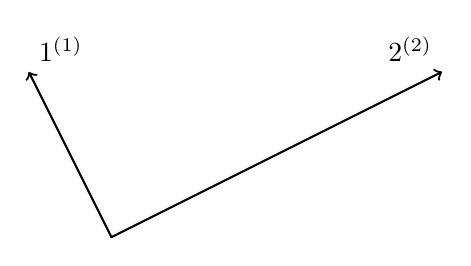
\begin{tikzpicture}[scale=2.1, line cap=round, line join=round]
            % two eigenvectors with different lengths
            \draw[->, thick] (0,0) -- (-0.5,1) node[above right] {$\eigval{1} \vu^{(1)}$};
            \draw[->, thick] (0,0) -- (2.0,1) node[above left]  {$\eigval{2} \vu^{(2)}$};
            \end{tikzpicture}
            \caption{The spectral decomposition of a \gls{normalmatrix} $\mA$ provides 
                     an orthonormal basis $\vu^{(1)}, \vu^{(2)}$. Applying $\mA$ 
                     amounts to a scaling of the basis \glspl{vector} by the 
                     \glspl{eigenvalue} $\eigval{1},\eigval{2}$.\label{fig:eigenvectors-length_dict}}
            \end{figure}
       Each basis element $\vu^{(\featureidx)}$ 
       is an \gls{eigenvector} of $\mA$ with corresponding \gls{eigenvalue} $\eigval{\featureidx}$, 
       for $\featureidx=1,\ldots,\nrfeatures$.
       },
	first={spectral decomposition},
    type=math,
	text={spectral decomposition}
}

\newglossaryentry{symmetricmatrix}
{name={symmetric matrix},
	description={A square\index{symmetric matrix} \gls{matrix} $\mA$ with real-valued 
                 entries that is equal to its transpose, i.e., $\mA=\mA^{T}$. Every 
                 symmetric \gls{matrix} is a \gls{normalmatrix}.},
	first={symmetric matrix},
	plural={symmetric matrices},
    type=math,
	firstplural={symmetric matrices},
	text={symmetric matrix}
}

\newglossaryentry{transpose}
{name={transpose},
 description={The transpose\index{transpose} of a real-valued \gls{matrix} is obtained by exchanging 
                  rows and columns. For a \gls{matrix} $\mA \in \mathbb{R}^{\samplesize \times \nrfeatures}$, 
				  its transpose is denoted $\mA^{T}$ and satisfies $\big(\mA^{T}\big)_{\featureidx,\featureidx'}=\mA_{featureidx',\featureidx}$.},
 	first={transpose},
    type=math, 
 	text={transpose}
 }

 \newglossaryentry{conjugatetranspose}
{name={conjugate transpose},
 description={The conjugate transpose\index{conjugate transpose} of a 
              \gls{matrix} is obtained by transposing the \gls{matrix} 
			  and taking the complex conjugate of each entry.
              For a matrix $\mA \in \mathbb{C}^{\samplesize \times \nrfeatures}$, its
              conjugate transpose is denoted by $\mA^{H} \in 
              \mathbb{C}^{\nrfeatures \times \samplesize}$ and is defined entrywise by
              \[
                 (\mA^{H})_{\featureidx,\sampleidx}
                 = \complexconjugate{\big(\mA\big)_{\sampleidx,\featureidx}},
              \]
              where $\complexconjugate{(\cdot)}$ denotes complex conjugation.},
 	first={conjugate transpose},
    type=math, 
 	text={conjugate transpose}
 }

\newglossaryentry{hermitian}
 {name={Hermitian (matrix)},
 	description={A square\index{Hermitian} matrix $\mA \in \mathbb{C}^{\nrfeatures \times \nrfeatures}$ is 
	             Hermitian if it coincides with its conjugate transpose, i.e., $\mA=\mA^{H}$. 
                 Trivally, a Hermitian matrix is also a \gls{normalmatrix}.},
 	first={Hermitian},
     type=math, 
 	plural={Hermitian},
 	firstplural={Hermitian},
 	text={Hermitian}
}

\newglossaryentry{dimension}
{name={dimension},
	description={The\index{dimension} dimension $\dim \mathcal{A}$ of a 
		\gls{vectorspace} $\mathcal{A}$ is the cardinality of any 
		\gls{basis} of $\mathcal{A}$ \cite{StrangLinAlg2016}. 
		Strictly speaking, this definition applies only to finite-dimensional \glspl{vectorspace}, 
		i.e., those that possess a finite \gls{basis}. 
		\begin{figure}[H]
			\begin{tikzpicture}[scale=1]
  			% Axes (optional; remove if you want it even more minimal)
  			%	\draw[->, thin, gray] (-0.2,0) -- (3.2,0) node[right] {$\vw^{(1)}$};
  			%	\draw[->, thin, gray] (0,-0.2) -- (0,3.2) node[above] {$\vw^{(1)}$};
  			\coordinate (O) at (0,0);
  			% Basis 1: standard (solid)
  			\draw[->, thick] (O) -- (1.8,0) node[below right] {$\ve^{(1)}$};
  			\draw[->, thick] (O) -- (0,1.6) node[above left] {$\ve^{(2)}$};
  			% Basis 2: rotated by ~45° (dashed)
			\draw[->, thick, dashed, shift={(3.5,0.5)}] (0,0) -- (1.2,1.2) node[above right] {$\vu^{(1)}$};
			\draw[->, thick, dashed, shift={(3.5,0.5)}] (0,0) -- (-1.2,1.2) node[above left] {$\vu^{(2)}$};
  			% Basis 3: non-orthogonal / skewed (dotted)
  			\draw[->, thick, dotted, shift={(-2.5,-2.5)}] (O) -- (2.0,0.6) node[above right] {$\vw^{(1)}$};
  			\draw[->, thick, dotted, shift={(-2.5,-2.5)}] (O) -- (0.4,1.8) node[left] {$\vw^{(2)}$};
  			% Simple legend
 			% \node[anchor=west] at (1.6,-0.6) {\footnotesize \textbf{Bases:} solid = standard,\; 
 			% dashed = rotated,\; dotted = skewed};
			\end{tikzpicture}
		\caption{Three \glspl{basis}, $\big\{\ve^{(1)},\ve^{(2)} \big\}, \big\{\vu^{(1)},\vu^{(2)} \big\},
		\big\{\vw^{(1)},\vw^{(2)} \big\}$, for the \gls{vectorspace} $\mathbb{R}^{2}$.} 
		\end{figure}
		For such spaces, all \glspl{basis} have the same cardinality, which is the dimension of the space 
		\cite[Ch.~2]{Axler2025}.	
   			 \\
		See also: \gls{vectorspace}, \gls{basis}. }, 
	text={dimension}, 
	type=math,
	first={dimension}  
}

\newglossaryentry{linearlyindep}
{name={linearly independent},
	description={A subset $\{\va^{(1)}, \,\ldots, \,\va^{(\nrfeatures)}\} \in \mathcal{V}$ 
		of a \gls{vectorspace} is linearly independent\index{linearly independent} 
		if there is no nontrivial linear combination of these \glspl{vector} that 
		equals the zero \gls{vector} \cite{StrangLinAlg2016}. 
		In other words, $$\sum_{\featureidx=1}^{\nrfeatures} \alpha_{\featureidx} \va^{(\featureidx)} = \mathbf{0}	
		\quad \text{ implies } \quad \alpha_{1} = \alpha_{2} = \ldots = \alpha_{k} = 0.$$ 
			\\ 
		See also: \gls{vectorspace}, \gls{vector}, \gls{dimension}, \gls{basis}.}, 
	text={linearly independent}, 
	type=math,
	first={linearly independent}  
}

\newglossaryentry{basis}
{name={basis},
	description={A basis\index{basis} of a \gls{vectorspace} $\mathcal{V}$ 
		is a set of \gls{linearlyindep} \glspl{vector} $\{\va^{(1)}, \,\ldots, \,\va^{(\nrfeatures)}\}$ such 
		that any \gls{vector} $\va \in \mathcal{A}$ can be expressed as a linear combination 
		of the basis \glspl{vector}, i.e.,	
		$$ \va = \sum_{\featureidx=1}^{\nrfeatures} \alpha_{\featureidx} \va^{(\featureidx)} 
		\quad \text{ for some } \alpha_{1}, \,\ldots, \,\alpha_{\nrfeatures} \in \mathbb{R}. $$
			\\
		See also: \gls{vectorspace}, \gls{linearlyindep}, \gls{vector}. },
	text={basis}, 
	firstplural={bases}, 
	plural={bases}, 
	type=math,
	first={basis} 
}

\newglossaryentry{widematrix}
{name={wide matrix},
	description={A\index{wide matrix} \gls{matrix} 
   		$\featuremtx \in \mathbb{R}^{\samplesize \times \nrfeatures}$ 
		is referred to as wide if it has more columns than rows, 
		i.e., when $\nrfeatures > \samplesize$.
		\begin{figure}[H]
			\centering
			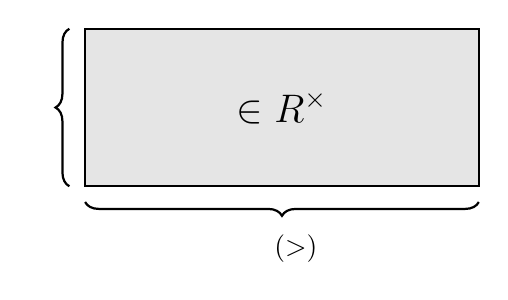
\begin{tikzpicture}
				\def\matHeight{2}
				\def\matWidth{5} 
				\draw[thick, fill=gray!20] (0,0) rectangle (\matWidth, \matHeight);
				\node at (0.5*\matWidth, 0.5*\matHeight) {\Large $\featuremtx \in \mathbb{R}^{\samplesize \times \nrfeatures}$};
				% vertical brace for samplesize (LEFT, correct orientation)
				\draw[decorate, decoration={brace, amplitude=5pt}, thick] 
  				(-0.2, 0) -- (-0.2, \matHeight)
  				node[midway, left=8pt] {$\samplesize$};
				\draw[decorate, decoration={brace, amplitude=5pt, mirror}, thick] 
        				(0, -0.2) -- (\matWidth, -0.2) 
        				node[midway, below=8pt] {$\nrfeatures \quad (\nrfeatures > \samplesize)$};
			\end{tikzpicture}
		\end{figure}
		See also: \gls{matrix}. },
	text={wide matrix}, 
	firstplural={wide matrices}, 
	plural={wide matrices}, 
	type=math,
   	first={wide matrix} 
}

\newglossaryentry{randomexperiment}
{name={random experiment},
	description={A random experiment\index{random experiment} is a physical (or abstract) process 
    	 	that produces an \gls{outcome} $\outcome$ from a set $\samplespace$ of possibilities. 
	 	This set of all possible \glspl{outcome} is referred to as the \gls{samplespace} of 
	 	the experiment. The key characteristic of a random experiment is that its 
	 	\gls{outcome} is unpredictable (or uncertain). Any measurement or observation 
	 	of the \gls{outcome} is a \gls{rv}, i.e., a \gls{function} of the \gls{outcome} $\outcome \in \samplespace$. 
	 	\Gls{probability} theory uses a \gls{probspace} as a mathematical structure for the study of 
	 	random experiments. A key conceptual property of a random experiment is that it can 
	 	be repeated under identical conditions. Strictly speaking, repeating a random experiment 
	 	a given number of $\samplesize$ times defines a new random experiment. The \glspl{outcome} 
	 	of this new experiment are length-$\samplesize$ sequences of \glspl{outcome} 
	 	from the original experiment (see Fig. \ref{fig_randomexperiment_dict}). While the \gls{outcome} of a single experiment is 
	 	uncertain, the long-run behaviour of the \glspl{outcome} of repeated experiments 
	 	tends to become increasingly predictable. This informal claim can be made 
	 	precise via fundamental results of \gls{probability} theory, such as the \gls{lln} 
	 	and the \gls{clt}.
	 	\begin{figure}[H]
		\begin{center}
	 		\begin{tikzpicture}[>=Stealth, node distance=1.5cm and 2cm, every node/.style={font=\small}]
			\node (experiment) [draw, rectangle, rounded corners, minimum width=2.6cm, align=center] {random\\experiment};
			\node (omega) [right=of experiment] {$\outcome \in \samplespace$};
			\coordinate (rightpad) at ($(omega.east) + (0.2,0)$);
			\draw[->] (experiment) -- (omega);
			\node (sequence) [below=of experiment, yshift=-0.5cm] {$(\outcome^{(1)}, \,\outcome^{(2)}, \,\dots, \,\outcome^{(\samplesize)})$};
			\node (sequence1) [below=of sequence, yshift=-0.5cm] {$(\datapoint^{(1)}, \,\datapoint^{(2)}, \,\dots, \,\datapoint^{(\samplesize)})$};
			\draw[->, thick] (experiment.south) -- node[midway, right, xshift=3pt] {repeat $\samplesize$ times} (sequence.north);
			\draw[->, thick] (sequence.south) -- node[midway, right, xshift=3pt] {\glspl{rv}} (sequence1.north);
			% Anchor node ~60% along the repeat arrow
			\path (experiment.south) -- (sequence.north) coordinate[pos=0.6] (repeatpoint);
			% Dotted rounded box enclosing experiment and part of repeat arrow
        			\node[draw=black, rounded corners, dotted, fit={(experiment) (repeatpoint) (rightpad)}, inner sep=8pt, label=above:{new random experiment with $\samplespace' = \samplespace \times \ldots \times \samplespace$}] {};
	 		\end{tikzpicture}
	     	\end{center}
		\caption{A random experiment produces an \gls{outcome} $\outcome \in \samplespace$ from a set 
			of possibilities (i.e., a \gls{samplespace}) 
			$\samplespace$. Repeating the experiment $\samplesize$ times yields another random 
			experiment, whose \glspl{outcome} are sequences 
			$(\outcome^{(1)}, \,\outcome^{(2)}, \,\dots, \,\outcome^{(\samplesize)}) \in \samplespace\times\ldots\times \samplespace$. 
			One example of a random experiment arising in many \gls{ml} applications is the gathering 
			of a \gls{trainset} $\datapoint^{(1)},\,\ldots,\,\datapoint^{(\samplesize)}$. \label{fig_randomexperiment_dict}}
	 	\end{figure} 
	 	Examples for random experiments arising in \gls{ml} applications include the following: 
	 	\begin{itemize} 
			\item \Gls{data} collection: The \glspl{datapoint} collected in \gls{erm}-based methods 
			can be interpreted as \glspl{rv}, i.e., as \glspl{function} of the \gls{outcome} $\outcome \in \samplespace$ 
			of a random experiment. 
			\item \Gls{stochGD} uses a random experiment at each iteration to select a subset of 
			the \gls{trainset}. 
			\item \Gls{privprot} methods use random experiments to perturb  
			the \glspl{output} of an \gls{ml} method to ensure \gls{diffpriv}. 
	 	\end{itemize} 
		See also: \gls{outcome}, \gls{samplespace}, \gls{rv}, \gls{probability}, \gls{probspace}.},
 	firstplural={random experiments},
 	plural={random experiments},
	type=math,
 	first={random experiment},
 	text={random experiment}
}

\newglossaryentry{pseudoinverse}
{name={pseudoinverse},
	description={The \index{pseudoinverse}Moore–Penrose pseudoinverse $\mA^{+}$ 
 		of a \gls{matrix} $\featuremtx \in \mathbb{R}^{\samplesize \times \nrfeatures}$ 
		generalizes the notion of an \gls{inverse} \cite{GolubVanLoanBook}. 
		The pseudoinverse arises naturally in \gls{ridgeregression} for a 
		\gls{dataset} with \gls{featuremtx} $\featuremtx$ and \gls{labelvec} 
		$\labelvec$ \cite[Ch.\ 3]{hastie01statisticallearning}. 
		The \glspl{modelparam} learned by \gls{ridgeregression} 
  		are given by
  		\[
  		\widehat{\weights}^{(\regparam)}  = \big(\featuremtx^{T} \featuremtx + \regparam \mI \big)^{-1} \featuremtx^{T} \vy, \quad \regparam > 0.
  		\]
  		We can then define the pseudoinverse $\featuremtx^{+} \in \mathbb{R}^{\nrfeatures \times \samplesize}$ via 
  		the limit \cite[Ch. 3]{benisrael2003generalized}
  		\[
  		\lim_{\regparam \to 0^+} \widehat{\weights}^{(\regparam)} = \featuremtx^+ \vy.
  		\]
		\\
		See also: \gls{matrix}, \gls{inverse}, \gls{ridgeregression}. },
 	first={pseudoinverse},
 	type=math, 
 	text={pseudoinverse}
} 

\newglossaryentry{tallmatrix}
{name={tall matrix},
	description={A\index{tall matrix} \gls{matrix} $\featuremtx \in \mathbb{R}^{\samplesize \times \nrfeatures}$ 
		is referred to as tall if it has more rows than columns, i.e., 
		when $\samplesize > \nrfeatures$.
		\begin{figure}[H]
			\centering
			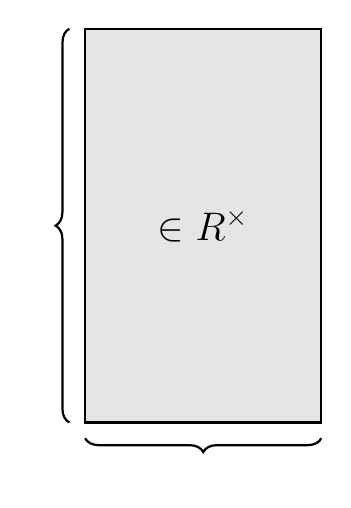
\begin{tikzpicture}
				\def\matHeight{5}
				\def\matWidth{3} 
				\draw[thick, fill=gray!20] (0,0) rectangle (\matWidth, \matHeight);
				\node at (0.5*\matWidth, 0.5*\matHeight) {\Large $\featuremtx \in \mathbb{R}^{\samplesize \times \nrfeatures}$};
				% vertical brace for samplesize (LEFT, correct orientation)
				\draw[decorate, decoration={brace, amplitude=5pt}, thick] 
  				(-0.2, 0) -- (-0.2, \matHeight)
  				node[midway, left=8pt] {$\samplesize$};
				\draw[decorate, decoration={brace, amplitude=5pt, mirror}, thick] 
        				(0, -0.2) -- (\matWidth, -0.2) 
        				node[midway, below=8pt] {$\nrfeatures$};
			\end{tikzpicture}
		\end{figure}
		See also: \gls{matrix}. },
	text={tall matrix}, 
	firstplural={tall matrices}, 
	plural={tall matrices}, 
	type=math,
   	first={tall matrix} 
}

\newglossaryentry{mgf}
{name={moment generating function (MGF)}, 
	description={Consider the\index{moment generating function (MGF)} MGF $\mgf{x}{t}$ 
	 	of a real-valued \gls{rv} $x$, which is defined as
	 	$\mgf{x}{t} = \expect \{ \exp(t \cdot x) \}$ for any $t \in \mathbb{R}$ 
	 	for which this \gls{expectation} exists \cite[Sec. 21]{BillingsleyProbMeasure}. 
		As its name indicates, the MGF allows us to compute the moments 
	 	$\expect\{ x^{k} \}$ for $k \in \mathbb{N}$. 
	 	In particular, the $k$th moment is obtained by evaluating the $k$th 
	 	derivative of $\mgf{x}{t}$ for $t=0$, i.e., $\expect\{ x^{k} \} = \mgfder{x}{k}{0}$. 
	 	This fact can be verified by the following identities: 
	 	\begin{align}
			\mgf{x}{t} & =\expect\{ \exp(t \cdot x)  \} \nonumber \\ 
			& \stackrel{(a)}{=} \expect\!\bigg\{\sum_{k=0}^{\infty} \frac{t^{k}}{k!} x^{k}\bigg\}  \nonumber \\ 
			& \stackrel{(b)}{=}  \sum_{k=0}^{\infty} \frac{t^{k}}{k!}\, \expect\!\big\{ x^{k} \big\}. \nonumber
	 	\end{align}
	 	Here, step $(a)$ is due to the Taylor series expansion of 
	 	$\exp\,(t \cdot x)$ and step $(b)$ is valid when the MGF exists 
	 	for all $t$ in some interval $(-t_{0},t_{0})$ \cite[p. 278]{BillingsleyProbMeasure}.
	 	\begin{figure}[H]
			\centering
			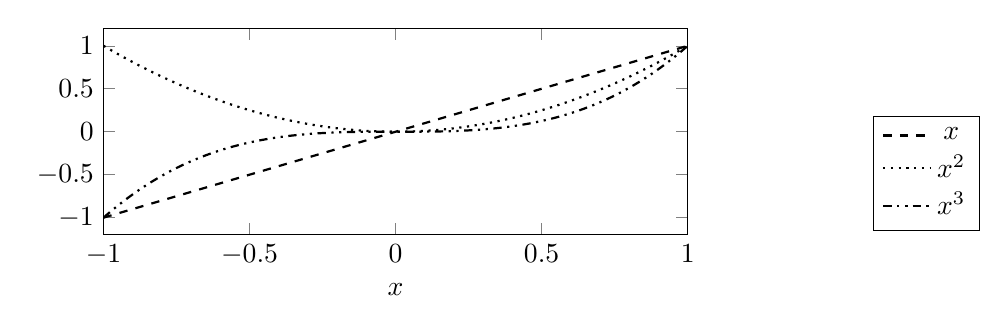
\begin{tikzpicture}
			\begin{axis}[
				width=9cm, height=4.2cm,
				domain=-1:1,
				samples=200,
				%axis lines*=left,        % removes bounding box, keeps left axis
				xlabel={$x$},
				ylabel={},
				ytick=\empty,
				ytick={-1,-0.5,0,0.5,1}, % manually set x-ticks
            			yticklabels={$-1$,$-0.5$,$0$,$0.5$,$1$},
				xtick={-1,-0.5,0,0.5,1}, % manually set x-ticks
            			xticklabels={$-1$,$-0.5$,$0$,$0.5$,$1$},
				xmin=-1, xmax=1,
				legend style={at={(1.5,0.02)},anchor=south east}
				]
				% f1 = x
				\addplot[thick, dashed] {x};
				\addlegendentry{$x$}
				% f2 = x^2
				\addplot[thick, dotted] {x^2};
				\addlegendentry{$x^{2}$}
				% f3 = x^3
				\addplot[thick, dashdotdotted] {x^3};
				\addlegendentry{$x^{3}$}
			\end{axis}
			\end{tikzpicture}
		\caption{The first few powers of an \gls{rv} $x$. The MGF 
			encodes the moments of $x$, which are the \glspl{expectation} 
			of the powers $x^{k}$ for $k=1,\,2,\,\ldots$.}
		\end{figure}
		The MGF is a useful tool for the study of sums of independent 
		\glspl{rv}. As a case in point, if $x$ and $y$ are independent 
		\glspl{rv}, then the MGF of their sum $z = x + y$ typically 
		satisfies $\mgf{z}{t} = \mgf{x}{t}\,\mgf{y}{t}$,
        		i.e., the MGF of the sum is typically the pointwise product of the 
		individual MGFs \cite[p.~280]{BillingsleyProbMeasure}.
		\\
 		See also: \gls{rv}, \gls{expectation}. }, 
 	first={moment generating function (MGF)}, 
 	firstplural={moment generating functions (MGFs)}, 
 	plural={MGFs}, 
 	type=math, 
 	text={MGF}
} 

\newglossaryentry{chernoffbound}
{name={Chernoff bound}, 
	description={The Chernoff bound\index{Chernoff bound} is a \gls{concentrationinequ} 
	             derived as a direct application of \gls{markovsinequality} \cite[Ch.\ 2]{vershynin2018high}. 
				 Let $\feature$ be a real-valued \gls{rv} such that its \gls{mgf} 
				 $\mgf{\feature}{t}=\expect\{\exp(t x)\}$ exists for some $t>0$. 
				 Applying \gls{markovsinequality} to the nonnegative 
				 \gls{rv} $\exp(t \feature)$ yields, for any $\eta\in\mathbb{R}$, 
				\begin{equation}
					\prob{ \feature \ge \eta }
					= \prob{ \exp(t \feature) \ge \exp(t\eta)}
					\le \exp(-t\eta)\, \expect\{\exp(t \feature)\}\nonumber.
				\end{equation}
				Note that this is actually an entire family of upper bounds, parametrized 
				by all valid choices for $t>0$ (i.e., $\mgf{\feature}{t}$ must exist). \\
	See also: \gls{markovsinequality}, \gls{chebyshevsinequality}, 
	\gls{hoeffdingsinequality}, \gls{concentrationinequ}.}, 
 	first={Chernoff bound}, 
 	type=math, 
 	text={Chernoff bound}
}

\newglossaryentry{rankdeficient}
{name={rank-deficient},
	description={A \gls{matrix} $\mA \in \mathbb{R}^{\samplesize \times \nrfeatures}$ 
         	is \gls{rank}-deficient\index{rank-deficient} if it is not \gls{fullrank}, i.e., 
         	when $\rank{\mA} < \min\{\samplesize,\nrfeatures\}$.
 		\begin{figure}[H]
			\begin{center}
			\begin{tikzpicture}[x=2cm]
				% LEFT: Standard basis vectors and unit square
				\begin{scope}
					\draw[->, thick] (0,0) -- (1,0) node[below] {$\vu^{(1)}$};
					\draw[->, thick] (0,0) -- (0,1) node[above] {$\vu^{(2)}$};
					%\draw[fill=gray!15] (0,0) -- (1,0) -- (1,1) -- (0,1) -- cycle;
					%\node at (0.5,0.5) {\small unit square};
					%\node at (0.5,-0.6) {standard basis};
				\end{scope}
				% RIGHT: Transformed basis vectors and parallelogram
				\begin{scope}[shift={(3.2,0)}]
				%\draw[->, thick] (0,0) -- (1,0) node[below] {$\vv^{(1)}$};
				%	\draw[->, thick] (0,0) -- (0,1) node[above] {$\vv^{(2)}$};
					\coordinate (A) at (0.2,0.0);
					\coordinate (B) at (2.0,0.0);
					\draw[->, very thick, red] (0,0) -- (A) node[below,yshift=-2pt] {$\mA \vu^{(1)}$};
					\draw[->, very thick, red] (0,0) -- (B) node[above,yshift=2pt] {$\mA \vu^{(2)}$};
					%	\node[blue] at (0.25,1.25) {};
					%	\node at (0.8,-0.6) {transformed basis};
				\end{scope}
				% Arrow between plots
				\draw[->, thick] (1.6,0.5) to[bend left] node[midway, above] {$\mA$} (2.7,0.5);
				%	\draw[->, thick] (1.3,0.5) -- (2.4,0.5) node[midway, above] {$\mA$};
			\end{tikzpicture}
			\end{center}
		\caption{Example of a \gls{rank}-deficient \gls{matrix} 
			$\mA \in \mathbb{R}^{2 \times 2}$.	\label{fig_matrix_rank_defdict}} 
		\end{figure} 
		In \gls{linreg}, the solution of the \gls{erm} problem is not 
		unique whenever the \gls{featuremtx} $\featuremtx$ is such that 
		the \gls{matrix} $\featuremtx^{\top}\featuremtx$ is \gls{rank}-deficient.
		\\
   		See also: \gls{fullrank}, \gls{dimension}, \gls{vectorspace}. }, 
	first={rank-deficient}, 
   	type=math,
   	text={rank-deficient}
}

\newglossaryentry{fullrank}
{name={full-rank},
 	description={A \gls{matrix} $\mA \in \mathbb{R}^{\samplesize \times \nrfeatures}$ 
  		is\index{full-rank} full-\gls{rank} if it has \gls{maximum} \gls{rank} \cite{StrangLinAlg2016}. 
  		For a \gls{tallmatrix}, i.e., when $\nrfeatures < \samplesize$, being 
  		full-\gls{rank} means that its \gls{rank} is equal to $\nrfeatures$. 
 		\begin{figure}[H]
			\centering
			\begin{tikzpicture}[every node/.style={font=\small}]
			% --- Full-rank square ---
			\node at (0,2) {$
			\mA =
			\begin{pmatrix}
			1 & 2\\
			3 & 4
			\end{pmatrix}
			$};
			\node[below=0.8cm of {$(0,2)$}] {\small full-\gls{rank} square};
			% --- Rank-deficient square ---
			\node at (4.5,2) {$
			\mB =
			\begin{pmatrix}
			1 & 2\\
			2 & 4
			\end{pmatrix}
			$};
			\node[below=0.8cm of {$(4.5,2)$}] {\small \gls{rankdeficient} square};
			% --- Full-rank tall (3x2) ---
			\node at (0,-1.0) {$
			\mC =
			\begin{pmatrix}
			1 & 0\\
			0 & 1\\
			1 & 1
			\end{pmatrix}
			$};
			\node[below=1.2cm of {$(0,-1.0)$}] {\small full-\gls{rank} \gls{tallmatrix}};
			% --- Rank-deficient wide (2x3) ---
			\node at (4.5,-1.0) {$
			\mD =
			\begin{pmatrix}
			1 & 2 & 3\\
			2 & 4 & 6
			\end{pmatrix}
			$};
			\node[below=1.2cm of {$(4.5,-1.0)$}] {\small \gls{rankdeficient} \gls{widematrix}};
			\end{tikzpicture}
		\caption{Examples of full-\gls{rank} and \gls{rankdeficient} \glspl{matrix}.}
		\end{figure} 
  		A square \gls{matrix} is full-\gls{rank} if and only if it is invertible. 
		\\ 
  		See also: \gls{matrix}, \gls{rank}, \gls{dimension}, \gls{linearmap}, \gls{columnspace}.}, 
	text = {full-rank}, 
  	type=math,
  	first={full-rank} 
 }

\newglossaryentry{rank}
{name={rank},
	description={The rank\index{rank} of a \gls{matrix} $\mA \in \mathbb{R}^{\samplesize \times \nrfeatures}$, 
 		denoted as $\rank{\mA}$, is the \gls{maximum} number of \gls{linearlyindep} columns 
 		of $\mA$ \cite{StrangLinAlg2016}. Equivalently, the rank can be defined as the 
 		\gls{dimension} of the \gls{columnspace} $\linspan{\mA} = \big\{ \mA \weights \mbox{ for some } 
 		\weights \in \mathbb{R}^{\nrfeatures} \big\}$. The rank of a \gls{matrix} 
 		$\mA \in \mathbb{R}^{\samplesize \times \nrfeatures}$ can neither exceed the 
 		number of rows nor the number of columns of $\mA$ \cite{Horn91}, \cite{MeyerMatrixAnalysis}, 
		i.e., $\rank{\mA} \leq \min \{ \samplesize, \nrfeatures \}$.  
		\\ 
 		See also: \gls{matrix}, \gls{dimension}, \gls{columnspace}, \gls{linearmap}.}, 
	text={rank}, 
	type=math,
	first={rank} 
}

\newglossaryentry{inverse}
{name={inverse matrix},
	description={An inverse \gls{matrix}\index{inverse matrix} $\mA^{-1}$ is defined for a 
 		square \gls{matrix} $\mA \in \mathbb{R}^{n \times n}$ that is of \gls{fullrank}, meaning its 
 		columns are linearly independent. In this case, $\mA$ is said to be invertible, 
 		and its inverse satisfies 
 		\[
 		\mA \mA^{-1} = \mA^{-1} \mA = \mI.
 		\]  	
     		A square \gls{matrix} is invertible if and only if its \gls{det} is nonzero. Inverse \glspl{matrix} are 
     		fundamental in solving systems of linear equations and in the closed-form solution of 
     		\gls{linreg} \cite{Strang2007}, \cite{Horn91}.  The concept of an inverse \gls{matrix} can be extended 
     		to \glspl{matrix} that are not square or do not have \gls{fullrank}. One may define a ``left inverse'' $\mB$ 
     		satisfying $\mB \mA = \mI$ or a ``right inverse'' $\mC$ satisfying $\mA \mC = \mI$. 
     		For general rectangular or singular \glspl{matrix}, the Moore–Penrose \gls{pseudoinverse}
     		$\mA^{+}$ provides a unified concept of a generalized inverse \gls{matrix} \cite{GolubVanLoanBook}.
 		 \begin{figure}[H]
 			\centering
 			\begin{tikzpicture}[x=2cm,y=2cm]
 			% LEFT: Standard basis
 			\begin{scope}
 				\draw[->, thick] (0,0) -- (1,0) node[below right] {$\vx$};
 				\draw[->, thick] (0,0) -- (0,1) node[above left] {$\vy$};
 			\end{scope}
 			% CENTER: Transformed basis (by A)
 			\begin{scope}[shift={(2.0,0)}]
 				\coordinate (A) at (1.5,0.5);
 				\coordinate (B) at (-0.2,1.2);
				\draw[->, very thick, red] (0,0) -- (A) node[pos=0.5, below right] {$\mA \vx$};
 				\draw[->, very thick, red] (0,0) -- (B) node[above right] {$\mA \vy$};
 			\end{scope}
 			% RIGHT: Inverse transformation
 			\begin{scope}[shift={(4.9,0)}]
 				\draw[->, very thick, blue] (0,0) -- (1,0) node[pos=0.5, below] {$\mA^{-1} (\mA \vx) = \vx$};
 				\draw[->, very thick, blue] (0,0) -- (0,1) node[above] {$\mA^{-1} (\mA \vy) = \vy$};
 			\end{scope}
 			% Curved arrows between stages
 			\draw[->, thick, bend left=20] (1.2,0.4) to node[above] {$\mA$} (1.8,0.4);
 			\draw[->, thick, bend left=20] (3.8,0.4) to node[below] {$\mA^{-1}$} (4.4,0.4);
 			\end{tikzpicture}
 		\caption{A \gls{matrix} $\mathbf{A}$ represents a linear transformation of $\mathbb{R}^{2}$. The inverse \gls{matrix} $\mathbf{A}^{-1}$ 
 			represents the inverse transformation. \label{fig_matrix_inverse_dict}} 
 		\end{figure}
		See also: \gls{matrix}, \gls{det}, \gls{linreg}, \gls{pseudoinverse}.},
	first={inverse matrix},
	type=math,
	text={inverse matrix}
}

\newglossaryentry{matrix}
{name={matrix},
	description={A matrix\index{matrix} of size $\samplesize \times \nrfeatures$ is a 2-D array of numbers, 
 		which is denoted by 
		$$
  		\mA = \begin{pmatrix}
   		A_{1,1} & A_{1,2} & \dots  & A_{1,\nrfeatures} \\
		A_{2,1} & A_{2,2} & \dots  & A_{2,\nrfeatures} \\
		\vdots  & \vdots  & \ddots & \vdots \\
		A_{\samplesize,1} & A_{\samplesize,2} & \dots  & A_{\samplesize,\nrfeatures}
		\end{pmatrix} \in \mathbb{R}^{\samplesize \times \nrfeatures}.
		$$
		Here, $A_{\sampleidx,\featureidx}$ denotes the matrix entry in the $\sampleidx$th row and the 
		$\featureidx$th column. Matrices are useful representations of various mathematical objects \cite{StrangLinAlg2016},
		including the following:
		\begin{itemize}
			\item Systems of linear equations: We can use a matrix to represent a system of linear equations 
			$$ \begin{pmatrix}
			A_{1,1} & A_{1,2} \\
			A_{2,1} & A_{2,2}
			\end{pmatrix}
			\begin{pmatrix}
				w_1 \\
				w_2
			\end{pmatrix}
			=\begin{pmatrix}
				y_1 \\
				y_2
			\end{pmatrix}
			\quad \text{ compactly as } \quad \mA \vw = \vy.
			$$
    			One important example of systems of linear equations is the optimality condition for the 
    			\glspl{modelparam} within \gls{linreg}. 
			\item \Glspl{linearmap}:
			Consider a $\nrfeatures$-dimensional \gls{vectorspace} $\mathcal{U}$ and a $\samplesize$-dimensional \gls{vectorspace} $\mathcal{V}$. 
			If we fix a \gls{basis} $\mathbf{u}^{(1)},\,\ldots,\,\mathbf{u}^{(\nrfeatures)}$ for $\mathcal{U}$ and a \gls{basis} $\mathbf{v}^{(1)},\,\ldots,\,\mathbf{v}^{(\samplesize)}$ 
			for $\mathcal{V}$, each matrix $\mA \in \mathbb{R}^{\samplesize \times \nrfeatures}$ naturally defines a 
			\gls{linearmap} $\alpha: \mathcal{U} \rightarrow \mathcal{V}$ (see Fig. \ref{fig_matrix_dict}) such that
   			$$\vu^{(\featureidx)} \mapsto \sum_{\sampleidx=1}^{\samplesize} A_{\sampleidx,\featureidx} \vv^{(\sampleidx)}.$$
			\item \Glspl{dataset}: We can use a matrix to represent a \gls{dataset}. Each row 
			corresponds to a single \gls{datapoint}, and each column corresponds to a specific 
			\gls{feature} or \gls{label} of a \gls{datapoint}. 
		\end{itemize}
		\begin{figure}[H]
		\begin{center}
		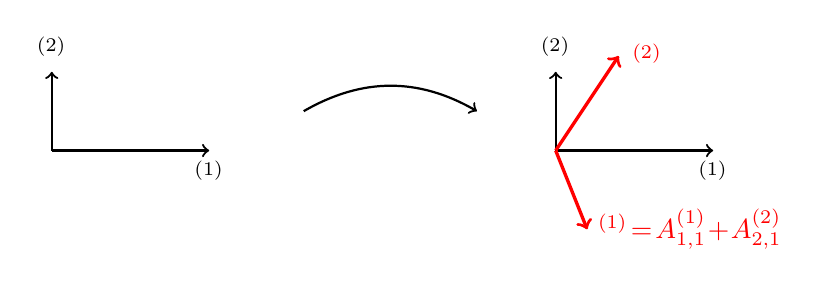
\begin{tikzpicture}[x=2cm]
			% LEFT: Standard basis vectors and unit square
			\begin{scope}
				\draw[->, thick] (0,0) -- (1,0) node[below] {$\vu^{(1)}$};
				\draw[->, thick] (0,0) -- (0,1) node[above] {$\vu^{(2)}$};
				%\draw[fill=gray!15] (0,0) -- (1,0) -- (1,1) -- (0,1) -- cycle;
				%\node at (0.5,0.5) {\small unit square};
				%\node at (0.5,-0.6) {standard basis};
			\end{scope}
			% RIGHT: Transformed basis vectors and parallelogram
			\begin{scope}[shift={(3.2,0)}]
				\draw[->, thick] (0,0) -- (1,0) node[below] {$\vv^{(1)}$};
				\draw[->, thick] (0,0) -- (0,1) node[above] {$\vv^{(2)}$};
				\coordinate (A) at (0.2,-1.0);
				\coordinate (B) at (0.4,1.2);
				\draw[->, very thick, red] (0,0) -- (A) node[below,right] {$\mA \vu^{(1)}\!=\!A_{1,1}\vv^{(1)}\!+\!A_{2,1}\vv^{(2)}$};
				\draw[->, very thick, red] (0,0) -- (B) node[right,xshift=1pt] {$\mA \vu^{(2)}$};
				%	\node[blue] at (0.25,1.25) {};
				%	\node at (0.8,-0.6) {transformed basis};
			\end{scope}
			% Arrow between plots
			\draw[->, thick] (1.6,0.5) to[bend left] node[midway, above] {$\mA$} (2.7,0.5);
		%	\draw[->, thick] (1.3,0.5) -- (2.4,0.5) node[midway, above] {$\mA$};
		\end{tikzpicture}
		\end{center}
		\caption{A matrix $\mA$ defines a \gls{linearmap} between two \glspl{vectorspace}. \label{fig_matrix_dict}} 
		\end{figure}
		See also: \gls{linearmap}, \gls{dataset}, \gls{linmodel}. },
	first={matrix},
	firstplural={matrices},
	type=math,
	plural={matrices},
	text={matrix}
}

\newglossaryentry{hyperplane}
{name={hyperplane},
	description={A hyperplane\index{hyperplane} is an $(\nrfeatures-1)$-dimensional affine 
		\gls{subspace} of a $\nrfeatures$-dimensional \gls{vectorspace}. In the 
		context of a \gls{euclidspace} $\mathbb{R}^{\nrfeatures}$, a 
		hyperplane is a set of the form
 		\[ 
		\{ \vx \in \mathbb{R}^\nrfeatures : \vw^\top \vx = b \}
  		\]
                 where $\vw \in \mathbb{R}^d \setminus \{0\}$ is a normal \gls{vector} 
                 and $b \in \mathbb{R}$ is an offset. Such a hyperplane partitions 
		$\mathbb{R}^\nrfeatures$ into two \glspl{halfspace}
		\[\{ \vx \in \mathbb{R}^\nrfeatures : \vw^\top \vx \leq b \} \quad 
		\text{and} \quad \{ \vx \in \mathbb{R}^\nrfeatures : \vw^\top \vx \geq b \}.\]
 		Hyperplanes arise as the \glspl{decisionboundary} of \glspl{linclass}.
		\\
		See also: \gls{subspace}, \gls{vectorspace}, \gls{euclidspace}, \gls{decisionboundary}. },
	first={hyperplane},
	type=math,
	plural={hyperplanes}, 
	firstplural={hyperplanes},
	text={hyperplane}
}

\newglossaryentry{normalvector}
{name={normal vector},
	description={See\index{normal vector} \gls{hyperplane}.},
	first={normal vector},
	type=math,
	plural={normal vectors}, 
	firstplural={normal vectors},
	text={normal vector}
}

\newglossaryentry{halfspace}
{name={halfspace},
	description={See\index{halfspace} \gls{hyperplane}.},
	first={halfspace},
	type=math,
	plural={halfspaces}, 
	firstplural={halfspaces},
	text={halfspace}
}

\newglossaryentry{subspace}
{name={subspace},
	description={A subset of a \gls{vectorspace} $\mathcal{V}$ is a subspace\index{subspace} of $\mathcal{V}$ if it is also a 
		\gls{vectorspace} with respect to the same operations as $\mathcal{V}$.
			   \\
		See also: \gls{vectorspace}.},
	type=math, 
	first={subspace},
	text={subspace}
}

\newglossaryentry{columnspace}
{name={column space},
	description={The column space\index{column space} of a \gls{matrix} 
		$\mA \in \mathbb{R}^{\samplesize \times \nrfeatures}$,
		denoted by $\linspan{\mA}$, is the set of all linear combinations of the 
		columns of $\mA$. In other words, 
		$$ \linspan{\mA} = \{ \mA \weights : \weights \in \mathbb{R}^{\nrfeatures} \}. $$
		The column space $\linspan{\mA}$ of the \gls{matrix} $\mA$ 
		is a \gls{subspace} of the \gls{euclidspace} $\mathbb{R}^{\samplesize}$.
			   \\
		See also: \gls{matrix}, \gls{vectorspace}.},
	type=math,
	first={column space},
	text={column space}
}

\newglossaryentry{mvndist}
{name={multivariate normal distribution}, 
	description={The\index{multivariate normal distribution} multivariate normal distribution, 
		which is denoted by $\mvnormal{\meanvecgeneric}{\covmtxgeneric}$, is a fundamental 
		\gls{probmodel} for numerical \glspl{featurevec} of fixed dimension $\nrfeatures$. 
		It defines a family of \glspl{probdist} over \gls{vector}-valued \glspl{rv} 
		$\featurevec \in \mathbb{R}^{\nrfeatures}$~\cite{BertsekasProb}, \cite{GrayProbBook}, \cite{Lapidoth09}. 
		Each distribution in this family is fully specified by its \gls{mean} \gls{vector} 
		$\meanvecgeneric \in \mathbb{R}^{\nrfeatures}$ and \gls{covmtx} 
		$\covmtxgeneric \in \mathbb{R}^{\nrfeatures \times \nrfeatures}$. When the 
		\gls{covmtx} $\covmtxgeneric$ is invertible, the corresponding \gls{probdist} is 
		characterized by the following \gls{pdf}:
		\[p(\featurevec) = 
 		\frac{1}{\sqrt{(2\pi)^{\nrfeatures} \det\,(\covmtxgeneric)}} 
 		\exp\left[ -\frac{1}{2} 
 		(\featurevec - \meanvecgeneric)\,^{T}\, \covmtxgeneric^{-1} 
 		(\featurevec - \meanvecgeneric) \right].
 		\]
		Note that this \gls{pdf} is only defined when $\covmtxgeneric$ is invertible.
   		More generally, any \gls{rv} $\featurevec \sim \mvnormal{\meanvecgeneric}{\covmtxgeneric}$ 
   		admits the following representation:
  		\[
    		\featurevec = \mA \vz + \meanvecgeneric
   		\]
   		where $\vz \sim \mvnormal{\mathbf{0}}{\mathbf{I}}$ is a \gls{stdnormvec} 
   		and $\mA \in \mathbb{R}^{\nrfeatures \times \nrfeatures}$ satisfies $\mA \mA^\top = \covmtxgeneric$. 
   		This representation remains valid even when $\covmtxgeneric$ is singular, in which case $\mA$ 
   		is not \gls{fullrank}~\cite[Ch. 23]{Lapidoth2017}.
   		The family of multivariate normal distributions is exceptional among \glspl{probmodel} for numerical 
   		quantities, at least for the following reasons. First, the family is closed under affine 
   		transformations, i.e.,
		\[ 
		\featurevec \sim \mathcal{N}(\meanvecgeneric,\covmtxgeneric) \mbox{ implies } 
		\mB\featurevec\!+\!\vc \sim \mathcal{N}\big( \mB\meanvecgeneric+\vc,\mB \covmtxgeneric \mB\,^{T} \big). 
		\]
		Second, the \gls{probdist} $\mathcal{N}(\mathbf{0},\covmtxgeneric)$ maximizes the 
		\gls{diffentropy} among all distributions with the same \gls{covmtx} $\covmtxgeneric$~\cite{coverthomas}. 
		\\ 
		See also: \gls{probmodel}, \gls{probdist}, \gls{stdnormvec}, \gls{diffentropy}, \gls{gaussrv}.}, 
	first={multivariate normal distribution},
	type=math, 
	text={multivariate normal distribution}
}

\newglossaryentry{stdnormvec}
{name={standard normal random vector}, 
	description={A\index{standard normal vector} standard normal random \gls{vector} is a random 
		\gls{vector} $\vx=\big(x_{1}, \,\ldots, \,x_{\nrfeatures}\big)\,^{T}$ 
		whose entries are \gls{iid} \glspl{gaussrv} $x_{\featureidx} \sim \mathcal{N}(0,1)$. 
		It is a special case of a \gls{mvndist}, $\vx \sim \mathcal(\mathbf{0},\mathbf{I})$.
		\\ 
		See also: \gls{vector}, \gls{iid}, \gls{gaussrv}, \gls{mvndist}, \gls{rv}.}, 
	first={standard normal random vector},
	type=math, 
	text={standard normal random vector}
}

\newglossaryentry{continuous}
{name={continuous}, 
	description={A \gls{function}\index{continuous} $f: \mathbb{R}^{\nrfeatures} \to \mathbb{R}$ is 
		continuous at a point $\featurevec' \in \mathbb{R}^{\nrfeatures}$ if, for 
	 	every $\epsilon > 0$, there is a $\delta > 0$ such that, for all 
	 	$\featurevec \in \mathbb{R}^{\nrfeatures}$ with $\normgeneric{\featurevec - \featurevec'}{2} < \delta$, 
	 	it holds that $|f(\featurevec) - f(\featurevec')| < \epsilon$ \cite{RudinBookPrinciplesMatheAnalysis}. 
	 	In other words, we can make $f(\featurevec)$ arbitrarily close to $f(\featurevec')$ 
	 	by choosing $\featurevec$ sufficiently close to $\featurevec'$. 
		\begin{figure}[H]
			\centering
	 		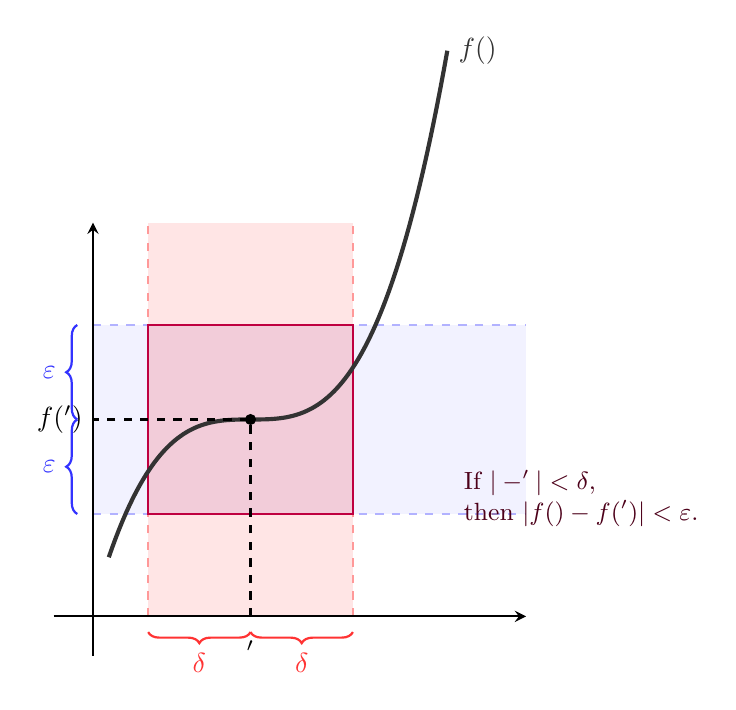
\begin{tikzpicture}[
				>=stealth, 
    				thick,
				%f(x) = 0.5(x-2)^3 + 2
    				declare function={f(\x) = 0.3*(\x-2)^3 + 2.5;}
				]
				\def\xprime{2}      % x'
    				\def\epsilonval{1.2}   % epsilon
				\def\deltaval{1.3}     % delta
				\def\xmax{5.5}
				\def\ymax{5}
				\fill[blue!5] (0, {f(\xprime)-\epsilonval}) rectangle (\xmax, {f(\xprime)+\epsilonval});
				\draw[blue!30, dashed] (0, {f(\xprime)-\epsilonval}) -- (\xmax, {f(\xprime)-\epsilonval});
				\draw[blue!30, dashed] (0, {f(\xprime)+\epsilonval}) -- (\xmax, {f(\xprime)+\epsilonval});
				\fill[red!10] ({\xprime-\deltaval}, 0) rectangle ({\xprime+\deltaval}, \ymax);
				\draw[red!40, dashed] ({\xprime-\deltaval}, 0) -- ({\xprime-\deltaval}, \ymax);
				\draw[red!40, dashed] ({\xprime+\deltaval}, 0) -- ({\xprime+\deltaval}, \ymax);
				\fill[purple!20] ({\xprime-\deltaval}, {f(\xprime)-\epsilonval}) rectangle ({\xprime+\deltaval}, {f(\xprime)+\epsilonval});
				\draw[purple, thick] ({\xprime-\deltaval}, {f(\xprime)-\epsilonval}) rectangle ({\xprime+\deltaval}, {f(\xprime)+\epsilonval});
				\draw[->] (-0.5,0) -- (\xmax,0) node[right] {$\feature$};
				\draw[->] (0,-0.5) -- (0,\ymax) node[above] {};
				% The Function 
				\draw[line width=1.5pt, black!80] plot[domain=0.2:4.5, samples=100] (\x, {f(\x)}) 
				node[right] {$f(\feature)$};
				\draw[dashed] (\xprime, 0) -- (\xprime, {f(\xprime)}) -- (0, {f(\xprime)});
				\fill[black] (\xprime, {f(\xprime)}) circle (2pt);
				\node[below,yshift=-5pt] at (\xprime, 0) {$\feature'$};
				\node[left] at (0, {f(\xprime)}) {$f(\feature')$};
				\draw[decorate, decoration={brace, amplitude=4pt}, blue!80] 
				(-0.2, {f(\xprime)}) -- (-0.2, {f(\xprime)+\epsilonval}) 
				node[midway, left=4pt] {$\varepsilon$};
				\draw[decorate, decoration={brace, amplitude=4pt}, blue!80] 
				(-0.2, {f(\xprime)-\epsilonval}) -- (-0.2, {f(\xprime)}) 
				node[midway, left=4pt] {$\varepsilon$};
				\draw[decorate, decoration={brace, amplitude=4pt, mirror}, red!80] 
				(\xprime, -0.2) -- ({\xprime+\deltaval}, -0.2) 
				node[midway, below=4pt] {$\delta$};
				\draw[decorate, decoration={brace, amplitude=4pt, mirror}, red!80] 
				({\xprime-\deltaval}, -0.2) -- (\xprime, -0.2) 
				node[midway, below=4pt] {$\delta$};
				\node[align=left, purple!40!black, font=\small] at (6.2, 1.5) 
				{If $| \feature - \feature' | < \delta$,\\
				then $| f(\feature) - f(\feature') | < \varepsilon$.};
			\end{tikzpicture}
		\caption{The \gls{function} $f(\feature) = 0.3(\feature-2)^3 + 2.5$ is continuous 
		         at every $\feature'$.}
		\end{figure}
		If $f$ is continuous at every point $\featurevec' \in \mathbb{R}^{\nrfeatures}$, then $f$ is said to be 
	 	continuous on $\mathbb{R}^{\nrfeatures}$. The notion of a continuous 
	 	\gls{function} can be naturally extended to \glspl{function} between general \glspl{metricspace} 
		\cite{RudinBookPrinciplesMatheAnalysis}.
		\\
		See also: \gls{euclidspace}, \gls{metric}.},
	first={continuous},
	type=math,
	text={continuous}
}

\newglossaryentry{minimum}
{name={minimum},
	description={Given a set of real numbers, the minimum\index{minimum} is the smallest of those numbers.
		Note that for some sets, such as the set of negative real numbers, the minimum does not exist.},
	firstplural={minima}, 
 	plural={minima},
	type=math, 
	first={minimum},
	text={minimum}
}

\newglossaryentry{co-domain}
{name={co-domain}, 
	description={The co-\gls{domain}\index{co-domain} of a \gls{function} 
		$f: \mathcal{U} \rightarrow \mathcal{V}$ is the set $\mathcal{V}$ 
		into which $f$ maps elements of its \gls{domain} $\mathcal{U}$.  
		\begin{figure}[H]
			\centering
			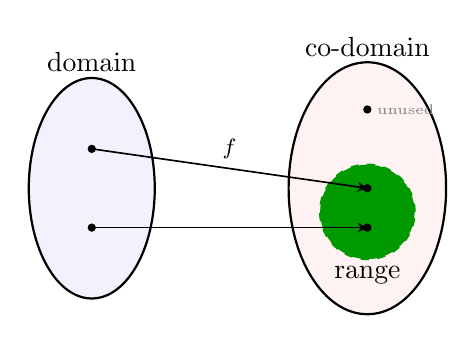
\begin{tikzpicture}[
			>=stealth, 
			node distance=2cm,
			scale=1.0, every node/.style={transform shape} % Scales the whole diagram down slightly
			]
			% Domain A
			\draw[thick, fill=blue!5] (0,0) ellipse (0.8cm and 1.4cm);
			\node[] at (0, 1.6) {\gls{domain}};
			% Codomain B
			\draw[thick, fill=red!5] (3.5,0) ellipse (1cm and 1.6cm);
			\node[] at (3.5, 1.8) {co-\gls{domain}};
			\draw[dashed, fill=green!10, thick, green!60!black] (3.5, -0.3) circle (0.6cm);
			\node[] at (3.5, -1.1) {range};
			\fill (0, 0.5) circle (1.5pt) coordinate (a1);
			\fill (0, -0.5) circle (1.5pt) coordinate (a2);
			% Output points
			\fill (3.5, 0) circle (1.5pt) coordinate (b1);
			\fill (3.5, -0.5) circle (1.5pt) coordinate (b2);
			% Unreached point
			\fill (3.5, 1.0) circle (1.5pt) coordinate (b_miss) node[right, font=\tiny, gray] {unused};
			\draw[->, semithick] (a1) -- (b1);
			\draw[->, semithick] (a2) -- (b2);
			% Function Label
			\node[font=\footnotesize] at (1.75, 0.5) {$f$};
			\end{tikzpicture}
		\end{figure}
		See also: \gls{domain}, \gls{function}, \gls{map}.},
	first={co-domain},
	firstplural={co-domains}, 
	type=math, 
	plural={co-domains},
	text={co-domain}
}

\newglossaryentry{cdf}
{name={cumulative distribution function (cdf)},
	description={The \index{cumulative distribution function (cdf)} cdf 
		$\cdf{\feature}{\eta}$ of a real-valued \gls{rv} $\feature$ is \cite{AshProbMeasure}, \cite{papoulis}
		$$\cdf{\feature}{\eta} \defeq \prob{\feature \leq \eta}.$$
					\\ 
		See also: \gls{rv}, \gls{pdf}, \gls{probdist}.},
	first={cumulative distribution function (cdf)},
	firstplural={cumulative distribution functions (cdfs)}, 
	plural={cdfs}, 
	type=math,
	text={cdf} 
}

\newglossaryentry{weightedgraph}
{name={weighted graph},
	description={A \gls{graph}\index{weighted graph} whose edges 
	are assigned numeric weights. Typically, these edge weights 
	are nonnegative real numbers. For example, if a \gls{graph} represents 
	a road network with nodes being intersections and edges representing 
	road segments, the edge weight could represent the capacity (measured 
	in maximum vehicles per hour) of the road segment \cite{NewmannBook}.  
	\begin{figure}[htbp] 
				\centering
			  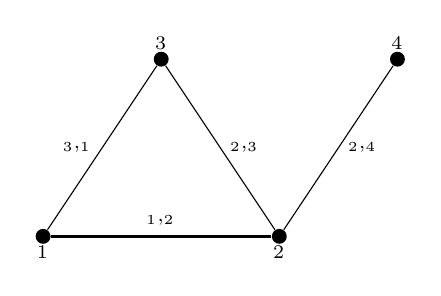
\begin{tikzpicture}[scale=1.5,
					node/.style={circle, fill=black, inner sep=1.9pt},
					lab/.style={anchor=west, xshift=3pt}
					]
					% Nodes (points)
					\node[node] (v1) at (0,0) {};
					\node[node] (v2) at (2,0) {};
					\node[node] (v3) at (1,1.5) {};
					\node[node] (v4) at (3,1.5) {};
					% Labels
					\node[anchor=north] at (v1) {$\nodeidx_1$};
					\node[anchor=north] at (v2) {$\nodeidx_2$};
					\node[anchor=south] at (v3) {$\nodeidx_3$};
					\node[anchor=south] at (v4) {$\nodeidx_4$};
					% Undirected edges
					\draw [line width=1pt] (v1) -- node[midway, above] {$\edgeweight_{\nodeidx_1,\nodeidx_2}$} (v2);
					\draw (v2) -- node[midway, right] {$\edgeweight_{\nodeidx_2,\nodeidx_3}$} (v3);
					\draw (v3) -- node[midway, left] {$\edgeweight_{\nodeidx_3,\nodeidx_1}$} (v1);
					\draw (v2) -- node[midway, right] {$\edgeweight_{\nodeidx_2,\nodeidx_4}$} (v4);
				\end{tikzpicture}
				\caption{A weighted graph with four nodes 
				$\nodes = \{\nodeidx_1, \nodeidx_2, \nodeidx_3, \nodeidx_4\}$ 
				and four edges $\edges = \{\{\nodeidx_1,\nodeidx_2\},
				\{\nodeidx_2,\nodeidx_3\}, \{\nodeidx_3,\nodeidx_1\}, 
				\{\nodeidx_2,\nodeidx_4\}\}$. Each edge is assigned a weight.}
			\end{figure}		
		See also: \gls{graph}.},
	first={weighted graph},
	type=math,
	firstplural={weighted graphs}, 
	plural={weighted graphs}, 
	text={weighted graph} 
}

\newglossaryentry{graph}
{name={graph},
 description={A graph\index{graph} $\graph = \pair{\nodes}{\edges}$ 
              consists of a node set $\nodes$ and an edge set $\edges$.
			  Each edge $\edgeidx \in \edges$ is characterized by the nodes to which 
			  it is connected and in what precise sense. For example, 
			  an edge of a \gls{directedgraph} is leaving one node 
			  and pointing to another node. An edge of an undirected 
			  graph connects two nodes without any sense of 
			  direction \cite{NewmannBook,RockNetworks}. 
			  In principle, there can also be several (parallel) edges that are 
			  connected to the same nodes in the same way \cite{RockNetworks}. 
			  Moreover, edges may connect a node to itself, resulting in 
			  so-called self-loops \cite{NewmannBook}. 
			  A simple undirected graph contains no 
			  parallel edges and no self-loops \cite{WilsonGraph2010}. 
			  Each edge $\edgeidx \in \edges$ of a simple undirected 
			  graph can be identified with a set of two nodes ${\nodeidx,\nodeidx'}$. 
			  \begin{figure}[htbp] 
				\centering
			  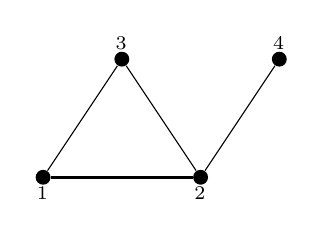
\begin{tikzpicture}[scale=1,
					node/.style={circle, fill=black, inner sep=1.9pt},
					lab/.style={anchor=west, xshift=3pt}
					]
					% Nodes (points)
					\node[node] (v1) at (0,0) {};
					\node[node] (v2) at (2,0) {};
					\node[node] (v3) at (1,1.5) {};
					\node[node] (v4) at (3,1.5) {};
					% Labels
					\node[anchor=north] at (v1) {$\nodeidx_1$};
					\node[anchor=north] at (v2) {$\nodeidx_2$};
					\node[anchor=south] at (v3) {$\nodeidx_3$};
					\node[anchor=south] at (v4) {$\nodeidx_4$};
					% Undirected edges
					\draw [line width=1pt] (v1) -- (v2);
					\draw (v2) -- (v3);
					\draw (v3) -- (v1);
					\draw (v2) -- (v4);
				\end{tikzpicture}
				\caption{A simple undirected graph with four nodes 
				$\nodes = \{\nodeidx_1, \nodeidx_2, \nodeidx_3, \nodeidx_4\}$ 
				and four edges $\edges = \{\{\nodeidx_1,\nodeidx_2\},
				\{\nodeidx_2,\nodeidx_3\}, \{\nodeidx_3,\nodeidx_1\}, 
				\{\nodeidx_2,\nodeidx_4\}\}$.}
			\end{figure}
		      \Glspl{weightedgraph} assign a numerical value $\edgeweight_{\edgeidx}$, 
			  referred to as edge weight, to each edge $\edgeidx \in \edges$.
					\\ 
		See also: \gls{map}, \gls{weights}.},
 first={graph},
 text={graph}, 
 firstplural={graphs}, 
 plural={graphs}, 
 type=math
}

\newglossaryentry{markovchain}
{name={Markov chain},
  description={A Markov chain\index{Markov chain} is a \gls{stochproc} $\{X_\timeidx \}_{\timeidx \in \mathbb{N}}$, 
               defined on a common \gls{probspace} and using the index set $\mathbb{N}$. The 
			   \gls{rv} $X_\timeidx$ might represent (the generation of) a state of a physical system 
			   at the time instant $\timeidx$. The defining property of a Markov chain 
			   is the Markov property \cite{NorrisMarkovChains1997,durrett2010probability,papoulis}: 
			   For all $\timeidx \in \mathbb{N}$,
 			   \begin{equation}
 				\nonumber \probdist^{(X_{\timeidx+1} \mid X_\timeidx,\ldots,X_1)} = \probdist^{(X_{\timeidx+1} \mid X_\timeidx)}. 
 				\end{equation}
 			    In other words, the \gls{condprobdist} of the next state $X_{\timeidx+1}$ 
				depends on the past $X_{\timeidx},X_{\timeidx-1},\dots,X_{1}$ 
				only through the current state $X_{\timeidx}$. The concept of a 
				Markov chain can be generalized from discrete time (with index set $\mathbb{N}$) 
				to continuous time (with index set $\mathbb{R}$) \cite{NorrisMarkovChains1997}. \\ 
				See also: \gls{stochproc}, \gls{condprobdist}.},
    first={Markov chain},
    type=math,
    text={Markov chain}, 
	plural={Markov chains}, 
	firstplural={Markov chains}
}

\newglossaryentry{markovprop}
{name={Markov property},
  description={See \gls{markovchain}\index{Markov property}.},
    first={Markov property},
    type=math,
    text={Markov property}
}

\newglossaryentry{em}
{name={expectation–maximization (EM)}, 
	description={\index{expectation–maximization (EM)}
	    The EM \gls{algorithm} \cite{dempster1977maximum} is an iterative \gls{optmethod} for 
		approximately solving certain \gls{maxlikelihood} \glspl{optproblem} 
		that are difficult to solve directly \cite[Sec. 9.4]{BishopBook}, \cite[Sec. 11.4.7]{Murphy2012}.
	    To motivate the EM \gls{algorithm} and explain its construction, 
		consider a \gls{ml} application involving a single observed \gls{datapoint} 
		with \gls{feature} $\feature \in \featurespace$, where $\featurespace$ 
		is a finite \gls{featurespace}. The \gls{data} generation 
		is modeled via a \gls{probmodel} that consists of a \gls{rv} $\feature'$ 
		with \gls{pmf} $\pmf{\feature'}{\cdot;\weights}$. Here, 
		the actual \glspl{modelparam} $\weights \in \paramspace$ - used for the \gls{data} 
		generation via sampling from $\pmf{\feature'}{\cdot;\weights}$ - are unknown. A widely 
		used approach for estimating these \glspl{modelparam} is via the solutions of the \gls{maxlikelihood} 
		problem
		\begin{equation}
			\label{equ_def_ML_EM_dict}
			\min_{\weights \in \paramspace} - \log \pmf{\feature'}{\feature;\weights}.
		\end{equation}
		For some \glspl{probmodel}, such as a \gls{gmm}, this \gls{optproblem} can be 
		difficult to solve directly. As a work-around, one can often introduce an auxiliary 
		attribute $\truelabel \in \labelspace$, generated via some \gls{rv} $\truelabel'$, 
		such that the corresponding \gls{probmodel} $\pmf{\feature',\truelabel'}{\cdot,\cdot;\weights}$ 
		yields a much easier \gls{maxlikelihood} problem 
		\begin{equation}
			\label{equ_def_complete_EM_dict}
			\min_{\weights \in \paramspace} 
			- \log \pmf{\feature',\truelabel'}{\feature,\truelabel;\weights}.
		\end{equation}
		The attribute $\truelabel$ is introduced solely to simplify 
		\eqref{equ_def_complete_EM_dict}, but it is not observed in practice—only the 
		feature $\feature$ is available. Thus, we cannot solve \eqref{equ_def_complete_EM_dict} 
		directly as we do not know which value $\truelabel$ to plug into the \gls{pmf} 
		$ \pmf{\feature',\truelabel'}{\feature,\truelabel;\weights}$. 
		The EM method resolves this dilemma by alternating between two steps:
		\begin{itemize}
			\item {\bf (E-step)} computing a “soft’’ estimate of the auxiliary 
			attribute $\truelabel$ in the form of the \gls{posterior} 
			$\pmf{\truelabel'|\feature'}{\cdot;\widehat{\weights}}$
			using the current choice $\widehat{\weights}$ for the \glspl{modelparam}, and 
			\item {\bf (M-step)} minimizing a surrogate \gls{objfunc} derived from this \gls{posterior}.
		\end{itemize}
		The completion of these two steps constitutes one full \gls{iteration} of 
		the EM method. 
		In more detail, the E-step produces the \gls{function}
		\[
		Q(\weights \mid \widehat{\weights})
		\defeq 
		- \sum_{\truelabel \in \labelspace} 
		\pmf{\truelabel'|\feature'}{\truelabel;\widehat{\weights}}
		\log\!\Big(
		\pmf{\feature',\truelabel'}{\feature,\truelabel;\weights}
		/\pmf{\truelabel'|\feature'}{\truelabel;\widehat{\weights}}
		\Big),
		\]
		and the M-step minimizes $Q(\weights \mid \widehat{\weights})$ over 
		$\weights \in \paramspace$.
		This \gls{function} satisfies two key properties \cite[Sec. 9.4]{BishopBook},\cite[Sec. 11.4.7]{Murphy2012}:
		\begin{itemize}
			\item {\bf Upper bound:}
			\begin{equation}
				\label{equ_upper_bound_EM_dict}
				Q(\weights\mid \widehat{\weights})
				\geq
				- \log \pmf{\feature'}{\feature;\weights}
				\quad \text{for all } \weights \in \paramspace.
			\end{equation}
			\item {\bf Tightness:}
			\begin{equation}
				\label{equ_upper_bound_EM_dict_tight}
				Q(\widehat{\weights}\mid \widehat{\weights})
				=- \log \pmf{\feature'}{\feature;\widehat{\weights}}.
			\end{equation}
		\end{itemize}
		To summarize, during each \gls{iteration}, EM minimizes an upper-bounding 
		surrogate \gls{objfunc} that is tight at the current iterate $\widehat{\weights}$. 
		Thus, EM is a \gls{majmin} method for approximately solving \eqref{equ_def_ML_EM_dict}. 
		The above construction and analysis of EM can be extended to more 
		general settings involving multiple \glspl{datapoint} 
		and infinite \glspl{featurespace} such as $\mathbb{R}^{\featuredim}$; see \cite[Sec. 11.4.7]{Murphy2012} for details. 
			\\
		See also: \gls{probmodel}, \gls{maxlikelihood}, \gls{optproblem}. },
	first={expectation–maximization (EM)},
	type=math, 
	text={EM}
}

\newglossaryentry{ppca}
{name={probabilistic principal component analysis (PPCA)}, 
	description={PPCA\index{probabilistic principal component analysis (PPCA)} 
		extends\linebreak basic \gls{pca} by using a \gls{probmodel} for \glspl{datapoint}. 
		The \gls{probmodel} of PPCA frames the task of \gls{dimred} 
		as an estimation problem that can be solved using \gls{em} \cite{TippingProbPCA}.
				\\
		See also: \gls{pca}, \gls{probmodel}, \gls{dimred}, \gls{em}.},
	first={probabilistic principal component analysis (PPCA)},
	type=math, 
	text={PPCA}
}

\newglossaryentry{condprobdist}
{name={conditional probability distribution}, 
	description={Consider\index{conditional probability distribution} 
     		a \gls{stochproc} consisting of two \glspl{rv} $\featurevec$ and $\truelabel$ 
    		with \gls{probdist} $\probdist^{(\featurevec,\truelabel)}$. The conditional 
    		\gls{probdist} of $\truelabel$ given (or conditioned on) $\featurevec$ is 
    		denoted by $\probdist^{(\truelabel\mid\featurevec)}$. It is defined via the 
    		\glspl{conditionalexpect} of the indicator \glspl{function} of  
    		\gls{measurable} sets in the \gls{sigmaalgebra} generated by 
    		the \gls{rv} $\truelabel$ \cite{BillingsleyProbMeasure}, \cite{KallenbergBook}.
		\\
		See also: \gls{probdist}, \gls{conditionalexpect}. },
  	first={conditional probability distribution}, 
  	plural={conditional probability distributions},
  	type=math, 
  	text={conditional probability distribution}
}

\newglossaryentry{linearmap}
{name={linear map}, plural={linear maps}, 
	description={A\index{linear map} linear \gls{map} 
		$f: \mathbb{R}^\nrfeatures \rightarrow \mathbb{R}^\samplesize$ 
	    	is a \gls{function} that satisfies additivity, i.e.,
		$f(\vx + \vy) = f(\vx) + f(\vy)$, and homogeneity, i.e.,
		$f(c\vx) = c f(\vx)$, for all \glspl{vector} $\vx, \vy \in \mathbb{R}^\nrfeatures$ 
		and scalars $c \in \mathbb{R}$. In particular, $f(\mathbf{0}) = \mathbf{0}$. 
		Any linear \gls{map} can be represented as a \gls{matrix} multiplication 
		$f(\vx) = \mA \vx$, for some \gls{matrix} $\mA \in \mathbb{R}^{m \times n}$. 
		The collection of real-valued linear \glspl{map} (where $\samplesize=1$), 
		for a given dimension $\nrfeatures$, constitute a \gls{linmodel}. The notion 
		of a linear \gls{map} can be generalized from the \gls{domain} $\mathbb{R}^{\nrfeatures}$ 
		and \gls{co-domain} $\mathbb{R}^{\samplesize}$ to arbitrary \glspl{vectorspace}.
		\\
		See also: \gls{map}, \gls{function}, \gls{vector}, \gls{matrix}, \gls{linmodel}.},
	first={linear map},
	type=math, 
	plural={linear maps}, 
	firstplural={linear maps}, 
	text={linear map}
}

\newglossaryentry{vector}
{name={vector},
	description={A\index{vector} vector is an element of a \gls{vectorspace}. 
		In the context of \gls{ml}, a particularly important example of a \gls{vectorspace} 
		is the \gls{euclidspace} $\mathbb{R}^{\nrfeatures}$, where $\nrfeatures \in \mathbb{N}$ 
		is the (finite) dimension of the space. A vector $\vx \in \mathbb{R}^{\nrfeatures}$ 
		can be represented as a list or one-dimensional (1-D) array of real numbers, i.e., 
		$x_1, \,\ldots, \,x_{\nrfeatures}$ with $x_\featureidx \in \mathbb{R}$ for 
		$\featureidx = 1, \,\ldots, \,\nrfeatures$. The value $x_\featureidx$ is the $\featureidx$th 
		entry of the vector $\vx$. It can also be useful to view a vector $\vx \in \mathbb{R}^{\nrfeatures}$ 
		as a \gls{function} that maps each index $\featureidx \in \{1, \,\ldots, \,\nrfeatures\}$ 
		to a value $x_\featureidx \in \mathbb{R}$, i.e., $\vx: \featureidx \mapsto x_\featureidx$. 
		This perspective is particularly useful for the study of \glspl{kernelmethod}. See Fig. 
		\ref{fig:vector-function-dual_dict} for the two views of a vector.
		\begin{figure}[H]
			% Left: Stem plot
			\begin{minipage}[c]{0.48\textwidth}
				\centering 
				2, --1, 3, 0, --2, 1
				\begin{minipage}{\textwidth}
				\vspace{5ex}
				\centering
				{\selectfont (a)}
				\end{minipage}
			\end{minipage}
			\hfill
			% Right: Column vector
			\begin{minipage}{0.48\textwidth}
			\centering
			\begin{tikzpicture}
			\begin{axis}[
    				width=6.5cm,
    				height=5cm,
    				title={},
    				xlabel={index $\featureidx$},
    				ylabel={$x_\featureidx$},
   		 		ymin=-3.5, ymax=3.5,
    				xmin=0.5, xmax=6.5,
   	 			xtick={1,2,3,4,5,6},
    				ytick={-3,-2,-1,0,1,2,3},
    				axis x line=bottom,        % <-- horizontal axis at y=0
    				axis y line=left,          % <-- vertical axis on the left
    				grid=both,
    				major grid style={dotted, gray!60},
    				enlargelimits=0.1
			]
			\addplot+[ycomb, thick, mark=*]
    			coordinates {
        				(1,2)
        				(2,-1)
       	 			(3,3)
        				(4,0)
        				(5,-2)
        				(6,1)
    			};
			\end{axis}
			\node at (2,-2.5) {(b)};
			\end{tikzpicture}
			\end{minipage}
		\caption{Two equivalent views of a vector $\vx= \big( 2, -1, 3, 0, -2, 1 \big)^{T} \in \mathbb{R}^{6}$.
			(a) As a numeric array. (b) As a \gls{map} $\featureidx \mapsto x_\featureidx$.}
			\label{fig:vector-function-dual_dict}
		\end{figure}
		See also: \gls{vectorspace}, \gls{euclidspace}, \gls{linearmap}.},
	first={vector},
	firstplural={vectors},
	type=math,
	plural={vectors},
	text={vector}
}

\newglossaryentry{vectorspace}
{name={vector space},
	description={A\index{vector space} \gls{vector} space $\mathcal{V}$ (also called linear space) 
		is a collection of elements, called \glspl{vector}, along with the following two operations 
		(see also Fig. \ref{fig:vector-ops_dict}): 
    		1) addition (denoted by $\vv+\vw$) of two \glspl{vector} $\vv,\vw$; and 2) multiplication 
		(denoted by $c \,\cdot \,\vv$) of a \gls{vector} $\vv$ with a scalar $c$ that belongs to some 
		number field (such as the real numbers $\mathbb{R}$ or the complex numbers $\mathbb{C}$). The defining 
		property of a \gls{vector} space is that it is closed under two specific operations. First, 
		if $\vv, \vw \in \mathcal{V}$, then $\vv + \vw \in \mathcal{V}$. Second, if $\vv \in \mathcal{V}$ 
		and $c \in \mathbb{R}$, then $c \vv \in \mathcal{V}$.
		\begin{figure}[H]
		\centering
			\begin{tikzpicture}[>=Stealth, scale=1.2]
			% Coordinates
  			\coordinate (O) at (0,0);            % Origin
  			\coordinate (V) at (2,1.5);          % vector v
  			\coordinate (W) at (1,3);            % vector w
  			\coordinate (VplusW) at (3,4.5);     % v + w
  			\coordinate (HalfV) at (1,0.75);     % 0.5 * v
  			\draw[->, thick, blue] (O) -- (V) node[pos=1, right] {$\vv$};
  			\draw[->, thick, red] (O) -- (W) node[pos=1, left] {$\vw$};
  			\draw[->, thick, purple] (O) -- (VplusW) node[pos=0.99, above right] {$\vv+\vw$};
  			\draw[dashed, red] (V) -- (VplusW);
  			\draw[dashed, blue] (W) -- (VplusW);
  			\draw[->, thick, orange] (O) -- (HalfV) node[midway, right] {$ \alpha \vv$};
			% Filled dots
  			\filldraw[black] (O) circle (2pt) node[below left] {$\mathbf{0}$};  % origin
  			\filldraw[blue] (V) circle (2pt);         % v
  			\filldraw[red] (W) circle (2pt);          % w
  			\filldraw[purple] (VplusW) circle (2pt);  % v + w
  			\filldraw[orange] (HalfV) circle (2pt);   % 0.5v
			\end{tikzpicture}
			\caption{A \gls{vector} space $\mathcal{V}$ is a collection of \glspl{vector} such that 
			scaling and adding them always yields another \gls{vector} in $\mathcal{V}$.}
			%In \gls{ml}, we use vector spaces to represent \glspl{rv}, \glspl{datapoint} 
			%(or their \glspl{featurevec}) as well as invariances (or symmetries) of \glspl{model}.}
			\label{fig:vector-ops_dict}
		\end{figure}
		A common example of a \gls{vector} space is the \gls{euclidspace} $\mathbb{R}^n$, which is 
		widely used in \gls{ml} to represent \glspl{dataset}. We can also use $\mathbb{R}^n$ 
		to represent, either exactly or approximately, the \gls{hypospace} used by an \gls{ml} method.  
		Another example of a \gls{vector} space, which is naturally associated with every \gls{probspace} 
		$\big(\samplespace,\eventspace,\prob{\cdot} \big)$, is the collection of all 
		real-valued \glspl{rv} $x: \samplespace \rightarrow \mathbb{R}$ \cite{RudinBook}, \cite{folland1999real}.  
		\\
		See also: \gls{vector}, \gls{euclidspace}, \gls{linmodel}, \gls{linearmap}.},
	first={vector space},
	plural={vector spaces}, 
	firstplural={vector spaces}, 
	type=math,
	text={vector space}
}

\newglossaryentry{stochastic}
{name={stochastic},
	description={We refer to a\index{stochastic} method as stochastic if it involves a 
		random component or is governed by probabilistic laws. \Gls{ml} methods use randomness 
		to reduce computational complexity (e.g., see \gls{stochGD}) or 
		to capture \gls{uncertainty} in \glspl{probmodel}.
		\\
		See also: \gls{stochGD}, \gls{uncertainty}, \gls{probmodel}.},
	first={stochastic},
	type=math, 
	text={stochastic}
}

\newglossaryentry{stochproc}
{name={stochastic process},
	description={A \gls{stochastic} process\index{stochastic process} is a collection of 
		\glspl{rv} defined on a common \gls{probspace} and indexed by some set 
		$\mathcal{I}$ \cite{GrayProbBook}, \cite{papoulis}, \cite{Brockwell91}. The index set 
		$\mathcal{I}$ typically represents time or space, allowing us to represent 
		random phenomena that evolve across time or spatial dimensions—for example, 
		sensor noise or financial time series. \Gls{stochastic} processes are not limited 
		to temporal or spatial settings. For instance, random \glspl{graph} such as 
		the \gls{ergraph} or the \gls{sbm} can also be viewed as \gls{stochastic} processes. 
		Here, the index set $\mathcal{I}$ consists of node pairs that index \glspl{rv} whose values 
		encode the presence or weight of an edge between two nodes. Moreover, \gls{stochastic} 
		processes naturally arise in the analysis of \glspl{stochalgorithm}, 
		such as \gls{stochGD}, which construct a \gls{sequence} of \glspl{rv}. 
		\\
		See also:  \gls{rv}, \gls{sbm}, \gls{stochGD}, \gls{uncertainty}, \gls{probmodel}.},
	first={stochastic process},
	firstplural={stochastic processes},
	type=math, 
	plural={stochastic processes},
	text={stochastic process}
}

\newglossaryentry{characteristicfunc}
{name={characteristic function},
	description={The characteristic \gls{function}\index{characteristic function} 
		of a real-valued \gls{rv} $x$ is the \gls{function} \cite[Sec. 26]{BillingsleyProbMeasure}
		$$ \phi_{x}(t) \defeq \expect { \exp\,(j t x) } \mbox{ with } j = \sqrt{-1}.$$
	 	The characteristic \gls{function} uniquely determines the \gls{probdist} of $x$. 
		\\
		See also: \gls{rv}, \gls{probdist}.},
	first={characteristic function},
	firstplural={characteristic functions}, 
	type=math, 
	plural={characteristic functions},
	text={characteristic function}
}

\newglossaryentry{entropy}
{name={entropy},
	description={Entropy\index{entropy} quantifies the \gls{uncertainty} or 
		unpredictability associated with an \gls{rv} \cite{coverthomas}. 
		For a \gls{discreteRV} $x$ taking on values in a finite set 
		$\mathcal{S} = \{x_1, \,\ldots, \,x_\nrcluster\}$ with 
		a \gls{pmf} $\pmf{x}{x_{\clusteridx}} (=\prob{x = x_{\clusteridx}})$, 
		the entropy is defined as \cite{coverthomas}
		\[
		   \entropy{x} \defeq -\sum_{\clusteridx=1}^{\nrcluster} \pmf{x}{x_{\clusteridx}}  \log \pmf{x}{x_{\clusteridx}} .
		\]
		For a given set of values $\mathcal{S}$, the entropy is maximized for a 
		uniformly distributed \gls{rv}, where $\pmf{x}{x_{\clusteridx}}=1/\nrcluster$. 
		The minimal entropy, which is zero, is obtained when $\pmf{x}{x_{\clusteridx}}=1$ 
		for some $x_{\clusteridx} \in \mathcal{S}$.
		\Gls{diffentropy} generalizes the concept of \gls{entropy} from \glspl{discreteRV} to 
		\gls{continuous} \glspl{rv}. 
		\\
		See also: \gls{uncertainty}, \gls{probmodel}.},
	first={entropy},
	type=math, 
	text={entropy}
}

\newglossaryentry{diffentropy}
{name={differential entropy},
	description={For\index{differential entropy} an 
		\gls{rv} $\featurevec \in \mathbb{R}^{\nrfeatures}$ 
		with a \gls{pdf} $\pdf{x}{\cdot}$, the differential \gls{entropy} 
		is defined as \cite{coverthomas}
		\[
		h(\featurevec) \defeq - \int_{\featurevec' \in \mathbb{R}^{\nrfeatures}} \log p(\featurevec') \, d \pdf{\featurevec}{\featurevec'} .
		\]
		Differential \gls{entropy} can be negative and lacks some properties of 
		\gls{entropy} for discrete-valued \glspl{rv}, such as invariance under 
		a change of variables \cite{coverthomas}. Among all \glspl{rv} with a 
		given \gls{mean} $\meanvecgeneric$ and \gls{covmtx} $\covmtxgeneric$, 
		$h(\featurevec)$ is maximized by $\featurevec \sim \mvnormal{\meanvecgeneric}{\covmtxgeneric}$. 
		\\
		See also: \gls{uncertainty}, \gls{probmodel}.},
	first={differential entropy},
	type=math,
	text={differential entropy}
}

\newglossaryentry{domain}
{name={domain}, 
	description={The domain\index{domain} of a \gls{function} 
		$f: \mathcal{U} \rightarrow \mathcal{V}$ is the set $\mathcal{U}$ 
		from which $f$ takes its inputs.  
		\\
		See also: \gls{function}, \gls{co-domain}, \gls{map}.},
	first={domain},
	firstplural={domains}, 
	type=math, 
	plural={domains},
	text={domain}
}

\newglossaryentry{function}
{name={function}, 
	description={A function\index{function} between two sets $\mathcal{U}$ and $\mathcal{V}$ assigns  
		each element $u \in \mathcal{U}$ exactly one element $f(u) \in \mathcal{V}$ \cite{RudinBookPrinciplesMatheAnalysis}.
		We write this as $$f: \mathcal{U} \rightarrow \mathcal{V}: u \mapsto f(u)$$ 
		where $\mathcal{U}$ is the \gls{domain} and $\mathcal{V}$ the \gls{co-domain} of $f$. 
		That is, a function $f$ defines a unique \gls{output} $f(u) \in \mathcal{V}$ for every 
		input $u \in \mathcal{U}$ (see Fig. \ref{fig_function_dict}).
		\begin{figure}[H]
			\centering
			\begin{tikzpicture}[>=stealth, node distance=1.2cm and 2.5cm]
				\tikzset{dot/.style={circle, fill=black, inner sep=1.2pt}}
				\node (A) [dot, label=left:$a$] {};
				\node (B) [dot, below=of A, label=left:$b$] {};
				\node (C) [dot, below=of B, label=left:$c$] {};
				\node (1) [dot, right=4cm of A, label=right:$\star$] {};
				\node (2) [dot, below=of 1, label=right:$\circ$] {};
				\node (3) [dot, below=of 2, label=right:$\otimes$] {};
				\node[draw=blue!70, thick, ellipse, inner sep=0.5cm, fit=(A)(B)(C), label=above:$\mathcal{U}$] {};
				\node[draw=green!70!black, thick, ellipse, inner sep=0.5cm, fit=(1)(2)(3), label=above:$\mathcal{V}$] {};
				\draw[->] (A) -- (2);
				\draw[->] (B) -- (1);
				\draw[->] (C) -- (2);
			\end{tikzpicture}
			\caption{A function \( f \colon \mathcal{U} \to \mathcal{V} \) mapping each element 
				of the \gls{domain} $\mathcal{U} =  \{a,b,c\}$ to exactly one element of 
				the \gls{co-domain} $\mathcal{V} = \{\star,\circ,\otimes\}$. \label{fig_function_dict}}
		\end{figure} 
		See also: \gls{domain}, \gls{co-domain}, \gls{output}. },
	first={function},
	firstplural={functions}, 
	type=math, 
	plural={functions},
	text={function}
}

\newglossaryentry{map}
{name={map}, 
	description={We\index{map} use the term map as a synonym for \gls{function}.
		\\
		See also: \gls{function}.},
	first={map},
	firstplural={maps},	
	type=math, 
	plural={maps},
	text={map}
}

\newglossaryentry{event}
{name={event}, 
	description={Consider\index{event} an \gls{rv} $\featurevec$, defined on some \gls{probspace}, 
		which takes values in a \gls{measurable} space $\featurespace$. An 
		event $\mathcal{A} \subseteq \featurespace$ is a subset of $\featurespace$ 
		such that the \gls{probability} $\prob{\featurevec \in \mathcal{A}}$ is well 
		defined. In other words, the \gls{preimage} $\featurevec^{-1}(\mathcal{A})$ 
		of an event belongs to the underlying \gls{sigmaalgebra}, i.e., the \gls{preimage} 
		is a \gls{measurable} subset of the \gls{samplespace} 
		\cite{RudinBook}, \cite{BillingsleyProbMeasure}, \cite{durrett2010probability}.	
		Roughly speaking, an event represents a set of possible \glspl{outcome} of some 
		process. One example of such a process could also be the treatment of a 
		health-care patient.
				\\
		See also: \gls{rv}, \gls{datapoint}, \gls{iidasspt}, \gls{probmodel}.},
	first={event},
	firstplural={events},
	plural={events},
	type=math,
	text={event} 
}

\newglossaryentry{countable}
{name={countable},
	description={A set is called countable\index{countable} if its 
		elements can be put into a one-to-one correspondence with the natural numbers 
		$\mathbb{N}=\{1,\,2,\,3,\,\ldots\}$ or with a finite subset of $\mathbb{N}$ \cite{HalmosSet}. 
		Equivalently, a set $\mathcal{A}$ is countable if there exists an \gls{injective} 
		\gls{function} $f:\mathcal{A}\rightarrow\mathbb{N}$. 
		\begin{figure}[H]
			\centering
			\begin{tikzpicture}[>=stealth, node distance=1.0cm, thick]
  			%--- Left: elements of set A ---
  			\node (a1) {$a_1$};
  			\node[below=of a1] (a2) {$a_2$};
  			\node[below=of a2] (a3) {$a_3$};
  			\node[left=0.4cm of a2, align=center] {$\mathcal{A}$};
  			% Ellipse enclosing set A
  			\begin{scope}[on background layer]
    			\draw[rounded corners, dashed, gray] ($(a1)+(-0.5,0.4)$) rectangle ($(a3)+(0.5,-0.4)$);
  			\end{scope}
  			%--- Right: natural numbers ---
  			\node[right=3.0cm of a1] (n1) {$1$};
  			\node[below=of n1] (n2) {$2$};
  			\node[below=of n2] (n3) {$3$};
  			\node[below=of n3] (n4) {$4$};
  			\node[below=of n4] (ndots) {$\vdots$};
  			\node[right=0.4cm of n2, align=center] {$\mathbb{N}$};
  			%--- Arrows (injective mapping) ---
  			\draw[->] (a1) -- (n3);
  			\draw[->] (a2) -- (n1);
  			\draw[->] (a3) -- (n4);
			\end{tikzpicture}
		\caption{An \gls{injective} \gls{function} that maps the elements of a finite set 
			$\mathcal{A}$ to the natural numbers $\mathbb{N}$, which implies that $\mathcal{A}$ is countable.}
		\end{figure}
		Typical examples include the set of integers $\mathbb{Z}$ and rational 
		numbers $\mathbb{Q}$. In contrast, the set of real numbers $\mathbb{R}$ 
		is not countable, meaning no such one-to-one correspondence with $\mathbb{N}$ exists.
		\\ 
		See also: \gls{injective}, \gls{function}.}, 
	first={countable}, 
	type=math, 
	text={countable}
}

\newglossaryentry{pmf}
{name={probability mass function (pmf)}, 
	description={The pmf\index{probability mass function (pmf)} 
		of a \gls{discreteRV} $\feature$ is a \gls{function} 
		$\pmf{\feature}{\cdot}: \featurespace \rightarrow [0,1]$ that assigns to each 
		possible value $\feature' \in \featurespace$ of the \gls{rv} $\feature$ 
		the \gls{probability} $\pmf{\feature}{\feature'} = \prob{\feature' = \feature}$ \cite{papoulis}. 
		Fig.\ \ref{fig_pmf_dict} illustrates the pmf of a \gls{discreteRV} $\feature$. 
		\begin{figure}[H]
			\centering
			\begin{tikzpicture}[>=stealth, thick,y=2cm]
  			\foreach \x/\p in {1/0.3, 4/0.7}{
			% Stem lines
			\draw[gray] (\x,0) -- (\x,\p);
			% Dots at the end of stems
			\fill[blue] (\x,\p) circle (2pt);
			% Labels next to each value
			% \node[anchor=west, blue] at (\x+0.1,\p) {\small $\pmf{\feature}{\cdot}$};
			}
  			\node[anchor=south,align=center] at (1,0.3) {\small $\pmf{\feature}{\star}=\frac{3}{10}$};
  			\node[anchor=north] at (1,0) {\small $\star$};
  			\node[anchor=north] at (4,0) {\small $\otimes$};
    			%--- Example datasets (same length, same frequencies, different permutations) ---
  			\node[anchor=west,text width=11cm] at (-1.2,-0.80) {
    			$\dataset = (\star,\,\star,\,\star,\,\otimes,\,\otimes,\,\otimes,\,\otimes,\,\otimes,\,\otimes,\,\otimes)$
  			};
  			\node[anchor=west,text width=11cm] at (-5.2,1.18) {\small
    			$\dataset' = (\otimes,\,\star,\,\otimes,\,\star,\,\otimes,\,\otimes,\,\star,\,\otimes,\,\otimes,\,\otimes)$
  			};
  			\node[anchor=west,text width=11cm] at (3.2,1.56) {
    			$\dataset'' = (\otimes,\,\otimes,\,\otimes,\,\star,\,\otimes,\,\star,\,\otimes,\,\otimes,\,\star,\,\otimes)$
  			};
			\end{tikzpicture}
		\caption{The pmf $\pmf{\feature}{\cdot}$ of a \gls{discreteRV} $\feature$ 
			taking values in the set $\featurespace = \{\star,\otimes\}$. Three \glspl{dataset} 
			are also shown whose relative frequencies of \glspl{datapoint} match 
			this pmf exactly. Such \glspl{dataset} could arise as \glspl{realization} of 
			\gls{iid} \glspl{rv} sharing the common pmf $\pmf{\feature}{\cdot}$. 
			\label{fig_pmf_dict}}
		\end{figure}
		A pmf always satisfies $\sum_{\feature' \in \featurespace} \pmf{\feature}{\feature'} = 1$. 
		We can view a pmf as representing a collection of (sufficiently long)  
		\glspl{dataset}. This collection contains any 
		$\dataset = \{\feature^{(1)}, \,\ldots, \,\feature^{(\samplesize)}\}$, 
		with the relative frequencies of every value $\feature' \in \featurespace$ 
		being close to the corresponding pmf value $\pmf{\feature}{\feature'}$, 
		$$ \frac{\big|\sampleidx \in \{1,\,\ldots,\,\samplesize\}: \feature^{(\sampleidx)}= \feature' \big|}
		{\samplesize} \approx \pmf{\feature}{\feature'}.$$ 
		Note that requiring relative frequencies to be close to the pmf values 
		implies that the empirical \gls{entropy} of such a \gls{dataset} is close to the 
		\gls{entropy} of the pmf $\pmf{\feature}{\cdot}$. Information theory refers 
		to the collection of such \glspl{dataset} as the typical set corresponding to the pmf 
		$\pmf{\feature}{\cdot}$ \cite{coverthomas}. A main result of information theory states 
		that a \gls{dataset} generated by \gls{iid} sampling from $\pmf{\feature}{\cdot}$ 
		belongs, with high \gls{probability}, to the typical set with respect to $\pmf{\feature}{\cdot}$ \cite[Th. 3.1.2]{coverthomas}.
				\\
		See also: \gls{discreteRV}, \gls{probability}, \gls{probdist}, \gls{probmodel}.},
	first={probability mass function (pmf)},
	firstplural={probability mass functions (pmfs)},
	plural={pmfs},
	type=math,
	text={pmf} 
}

\newglossaryentry{discreteRV}
{name={discrete random variable (discrete RV)}, 
 	description={A\index{discrete random variable (discrete RV)} \gls{rv}, i.e., 
		a \gls{function} that maps the \glspl{outcome} of a \gls{randomexperiment} 
		to elements of a \gls{measurable} space $\featurespace$, 
		is referred to as discrete if its value space 
		$\featurespace$ \gls{countable} \cite{BillingsleyProbMeasure}. 
			\\
		See also: \gls{rv}, \gls{probability}, \gls{probdist}.},
 	first={discrete random variable (discrete RV)},
	firstplural={discrete random variables (discrete RVs)}, 
	plural={discrete RVs},
	type=math, 
 	text={discrete RV}  
}

\newglossaryentry{rv}
{name={random variable (RV)}, plural={RVs},
 	description={An RV\index{random variable (RV)} is a \gls{function} that maps the 
		\glspl{outcome} of a \gls{randomexperiment} to elements of a \gls{measurable} space 
		\cite{BillingsleyProbMeasure}, \cite{GrayProbBook}. 
 		Mathematically, an RV is a \gls{function} $x: \samplespace \rightarrow \featurespace$ 
		whose \gls{domain} is the \gls{samplespace} $\samplespace$ of a \gls{probspace} and 
		whose \gls{co-domain} is a \gls{measurable} space $\featurespace$. 
 		Different types of RVs include  
 		\begin{itemize} 
 			\item {binary RVs}, which map each \gls{outcome} to an element of a binary 
			set (e.g., $\{-1,1\}$ or $\{\text{cat}, \text{no cat}\}$); 
			\item {\glspl{discreteRV}}, which take on values in a \gls{countable} set (which can 
			be finite or countably infinite); 
 			\item {real-valued RVs}, which take on values in the real numbers $\mathbb{R}$;  
 			\item {\gls{vector}-valued RVs}, which map \glspl{outcome} to the \gls{euclidspace} $\mathbb{R}^{\featuredim}$.  
 		\end{itemize} 
 		\Gls{probability} theory uses the concept of \gls{measurable} spaces to rigorously define 
 		and study the properties of collections of RVs \cite{BillingsleyProbMeasure}.
			\\
		See also: \gls{function}, \gls{randomexperiment}, \gls{samplespace}, \gls{probspace}, \gls{vector}, \gls{euclidspace}, \gls{probability}, \gls{measurable}.}, 
	first={random variable (RV)},
	firstplural={random variables (RVs)},
	plural={RVs},
	text={RV}  
}

\newglossaryentry{outcome}
{name={outcome}, 
  	description={Outcome is one possible\index{outcome} result of a physical process.  
		Such a process could be the observation of a physical phenomenon,  
		a computation performed by an \gls{algorithm}, or a \gls{randomexperiment}  
		\cite{BillingsleyProbMeasure}.   
		\\
 		See also: \gls{samplespace}.},  
	type=math, 
  	first={outcome}, 
 	firstplural={outcomes},
 	plural={outcomes},
  	text={outcome}
}

\newglossaryentry{probspace}
{name={probability space}, 
 	description={A\index{probability space} \gls{probability} space is a mathematical 
 		structure that allows us to reason about a \gls{randomexperiment}, e.g., 
		the observation of a physical phenomenon. 
 	   	Formally, a \gls{probability} space $\mathcal{P}$ is a triplet 
		$(\samplespace, \eventspace, \prob{\cdot})$ where
 		\begin{itemize} 
 			\item  $\samplespace$ is a \gls{samplespace} containing all possible \glspl{outcome} 
			of a \gls{randomexperiment};
 			\item  $\eventspace$ is a \gls{sigmaalgebra}, i.e., a collection of subsets of 
			$\samplespace$ (called \glspl{event}) that satisfies certain closure properties 
			under set operations;
 			\item $\prob{\cdot}$ is a \gls{probdist}, i.e., a \gls{function} that assigns 
			a \gls{probability} $\prob{\mathcal{A}} \in [0,1]$ to each \gls{event} $\mathcal{A} 
			\in \eventspace$. This \gls{function} must satisfy $\prob{\samplespace} = 1$ and 
			$\prob{\bigcup_{i=1}^{\infty} \mathcal{A}_i} = \sum_{i=1}^{\infty} \prob{\mathcal{A}_i}$ 
			for any \gls{countable} \gls{sequence} of pairwise disjoint \glspl{event} $\mathcal{A}_1, \,\mathcal{A}_2, \,\ldots$ in $\mathcal{F}$.
 		\end{itemize}
 		\Gls{probability} spaces provide the foundation of \glspl{probmodel} 
		that can be used to study the behavior of \gls{ml} methods \cite{BillingsleyProbMeasure}, \cite{GrayProbBook}, \cite{ross2013first}.
				\\
		See also: \gls{probability}, \gls{randomexperiment}, \gls{samplespace}, \gls{event}, \gls{probdist}, \gls{function}, \gls{probmodel}, \gls{ml}.},  
 	first={probability space}, 
	plural={probability spaces},
	firstplural={probability spaces},
	type=math, 
 	text={probability space}
}

\newglossaryentry{integrable}
{name={integrable},
	description={A \gls{measurable} \gls{function} $f\!:\!\samplespace \!\to\! \mathbb{R}$ 
		defined on a \gls{measurespace} $(\samplespace, \,\sigmaalgebra, \,\mu)$ 
		is called integrable\index{integrable} if the \gls{LebesgueIntegral} 
		of its absolute value is finite, i.e.,
		\[
		\int_{\samplespace} |f(x)|\,\mathrm{d}\mu < \infty.
		\]
		In this case, the \gls{LebesgueIntegral} $\int_{\samplespace} f(x)\,\mathrm{d}\mu$ 
		is well-defined and finite. An \gls{rv} $x$ defined on the \gls{samplespace} 
		of a \gls{probspace} $(\samplespace, \,\sigmaalgebra, \,\probdist)$ 
		is integrable if 
		\[
		\expect\{|x|\}
		= \int_{\samplespace} |x(\omega)|\,\mathrm{d}\probdist 
		< \infty
		\]
		which ensures that the \gls{expectation} $\expect\{|x|\}$ 
		exists and is finite. 
		\\ 
		See also: \gls{measurespace}, \gls{measure}.},
	first={integrable},
	type=math, 
	text={integrable}
}

\newglossaryentry{measurespace}
{name={measure space},
	description={A \gls{measure} space\index{measure space} is a triple $(\samplespace, \,\sigmaalgebra, \,\mu)$ consisting of 
        		a set $\samplespace$, a \gls{sigmaalgebra} $\sigmaalgebra$ of subsets 
		of $\samplespace$, and a \gls{measure} $\mu\!:\sigmaalgebra\!\to\![0,\infty)$. 
        		The \gls{measure} $\mu$ assigns a nonnegative number to each \gls{measurable} 
		set $\mathcal{A} \in \sigmaalgebra$, generalizing the 
		notions of length, area, or volume in \glspl{euclidspace} \cite{RudinBookPrinciplesMatheAnalysis}, \cite{HalmosMeasure}. 
		\Gls{measure} spaces provide the mathematical foundation for the 
		\gls{LebesgueIntegral} or the definition of \glspl{rv} as \gls{measurable} mappings 
        		between \gls{measure} spaces.  
        		A \gls{probspace} is a special case of a \gls{measure} space 
		where the total \gls{measure} of the \gls{samplespace} is normalized to one, 
        		i.e., $\mu(\samplespace) = 1$. In this case, $\mu$ is called a \gls{probdist}.
		\\ 
		See also: \gls{measurable}, \gls{probspace}, \gls{probdist}. },
    	first={measure space},
	plural={measure spaces}, 
	firstplural={measure spaces}, 
	type=math, 
    	text={measure space}
}

\newglossaryentry{measure}
{name={measure},
	description={A measure\index{measure} $\mu$ on a set $\samplespace$ equipped with a 
		\gls{sigmaalgebra} $\sigmaalgebra$ is a \gls{function} $\mu: \sigmaalgebra \to [0, \infty)$ 
		that assigns a nonnegative value to each \gls{measurable} set 
		$\mathcal{A} \in \sigmaalgebra$ such that 
		\cite{RudinBookPrinciplesMatheAnalysis}, \cite{BillingsleyProbMeasure}, \cite{HalmosMeasure}: 
		1) $\mu(\emptyset) = 0$; and 
		2) for any \gls{countable} collection $\{\mathcal{A}_i\}_{i=1}^{\infty}$ of 
		pairwise disjoint sets in $\sigmaalgebra$,
		\[
		\mu\!\left(\bigcup_{i=1}^{\infty} A_i\right) = \sum_{i=1}^{\infty} \mu(A_i)
		\]
		which is referred to as ``\gls{countable} additivity''.
		\\
		See also: \gls{measurable}, \gls{countable}. },
	first={measure},
	type=math, 
	plural={measures}, 
	firstplural={measures}, 
	text={measure}
}

\newglossaryentry{LebesgueIntegral}
{name={Lebesgue integral},
	description={The Lebesgue integral\index{Lebesgue integral} 
		assigns each \gls{integrable} \gls{function} 
		$f: \mathbb{R}^{\nrfeatures} \rightarrow \mathbb{R}$ a number 
		$\int_{\featurevec} f(\featurevec) d\featurevec$ 
		that is referred to as the integral of $f$. 
		The integral of $f$ can be interpreted as the volume that 
		is enclosed by the \gls{function} $f$ in the space 
		$\mathbb{R}^{\nrfeatures+1}$. We can compute it be increasingly 
		accurate approximations by \glspl{simplefunction} 
		\cite[Ch. 1]{RudinBook}. 
		\begin{figure}[H]
			\centering
			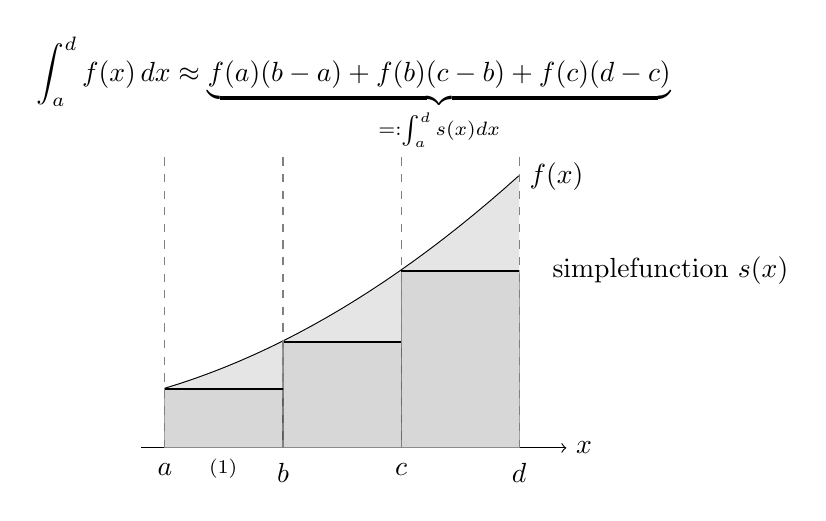
\begin{tikzpicture}[scale=1.5]
  			% Axes
  			\draw[->] (-0.2,0) -- (3.4,0) node[right] {$x$};
 			% \draw[->] (0,-0.1) -- (0,2.6) node[above] {$y$};
  			% Continuous function f(x)
  			\draw[thick,domain=0:3,smooth] plot(\x,{0.5+0.3*\x+0.1*\x*\x}) node[right] {$f(x)$};
  			% Shade area under f(x)
  			\fill[gray!20] (0,0) -- plot[domain=0:3] (\x,{0.5+0.3*\x+0.1*\x*\x}) -- (3,0) -- cycle;
  			% Lower simple function: left-endpoint rectangles for [0,1], [1,2], [2,3]
  			\draw[fill=gray!50,opacity=0.35] (0,0) rectangle (1,0.5);
  			\node at (0.5,-0.2) {$\cluster^{(1)}$}; 
  			\draw[fill=gray!50,opacity=0.35] (1,0) rectangle (2,0.9);
  			\draw[fill=gray!50,opacity=0.35] (2,0) rectangle (3,1.5);
  			% Step lines of the simple function
  			\draw[thick] (0,0.5)--(1,0.5);
  			\draw[thick] (1,0.9)--(2,0.9);
  			\draw[thick] (2,1.5)--(3,1.5);
 	 		\node[above left] at (0.8,0.5) {};
  			% Dashed partition lines
  			\foreach \x in {0,1,2,3} \draw[dashed,gray] (\x,0) -- (\x,2.5);
  			% Labels
  			\node[anchor=north] at (0,-0.05) {$a$};
  			\node[anchor=north] at (1,-0.05) {$b$};
  			\node[anchor=north] at (2,-0.05) {$c$};
  			\node[anchor=north] at (3,-0.05) {$d$};
  			\node at (1.6,3.0) {$\displaystyle \int_a^d f(x)\,dx \approx \underbrace{f(a)(b-a) + f(b)(c-b)+f(c)(d-c)}_{=:\int_a^d s(x)dx}$};
  			\node [anchor=west] at (3.2,1.5) {\gls{simplefunction} $s(x)$};
			\end{tikzpicture}
		\end{figure}
 		It is useful to think of the Lebesgue integral as a \gls{function} that maps 
 		an \gls{integrable} \gls{function} $f$ to the value of its integral, 
		$$ f \mapsto \int_{\featurevec} f(\featurevec) d\featurevec.$$ 
		The precise definition of this \gls{function}, whose \gls{domain} 
		consists of the \gls{integrable} \glspl{function}, is a cornerstone of 
		\gls{measure} theory \cite[Ch. 1]{RudinBook}.
					\\ 
		See also: \gls{function}.},
	first={Lebesgue integral},
	text={Lebesgue integral},
	type=math, 
	plural={Lebesgue integrals},
	firstplural={Lebesgue integrals}
}

\newglossaryentry{conditionalexpect}
{name={conditional expectation}, 
	description={Consider a numeric \gls{rv} $\featurevec \in \mathbb{R}^{\nrfeatures}$ defined on a 
                 \gls{probspace} $\mathcal{P}=(\samplespace,\,\eventspace,\,\probmeasure)$. 
                 Let $\sigmaalgebra' \subseteq \sigmaalgebra$ be a (sub-)\gls{sigmaalgebra} that 
                 represents partial information about the \gls{outcome} of a \gls{randomexperiment}. 
                 The conditional \gls{expectation}\index{conditional expectation} of 
                 $\featurevec$ given (or conditioned on) $\sigmaalgebra'$, denoted 
                 $\expect\{ \featurevec \mid \sigmaalgebra'\}$, is a numeric \gls{rv} 
		that \cite{BillingsleyProbMeasure}, \cite{durrett2010probability}:
                	1) is \gls{measurable} with respect to $\sigmaalgebra'$; and
                 2) satisfies
		$$
    		\int_{\mathcal{A}} \expect\{\featurevec \mid \sigmaalgebra'\} {\rm d} \probmeasure =
    		\int_{\mathcal{A}} \featurevec {\rm d} \probmeasure \quad \text{for any } \mathcal{A} \in \sigmaalgebra'.
		$$
               	Intuitively, $\expect\{\featurevec \mid \eventspace'\}$ summarizes 
               	the average value of $\featurevec$ using only information contained 
               	in the (typically smaller) \gls{sigmaalgebra} $\sigmaalgebra'$ 
		\cite{BillingsleyProbMeasure}, \cite{GrayProbBook}, \cite{ross2013first}. 
		\\
              	See also: \gls{probspace}, \gls{sigmaalgebra}, \gls{expectation}.}, 
 	first={conditional expectation},
 	plural={conditional expectations}, 
 	type=math, 
 	firstplural={conditional expectations},  
 	text={conditional expectation}
}

\newglossaryentry{conditionalpmf}
{name={conditional probability mass function (conditional pmf)}, 
	description={Consider two \glspl{discreteRV} $\truelabel$ and $\feature$ defined on 
                  the same \gls{probspace} $(\samplespace,\eventspace,\prob{\cdot})$. 
                  The conditional pmf\index{conditional pmf} of $\truelabel$ given 
				  (or conditioned on) $\feature$ is denoted 
                $\pmf{\truelabel \mid \feature}{\cdot \mid \cdot}$ and is defined by
                \[
                  \pmf{\truelabel \mid \feature}{\truelabel' \mid \feature'}
                  :=
                  \prob{\truelabel=\truelabel' \mid \feature=\feature'},
               \]
                for all realizations $\truelabel',\feature'$ with 
                $\prob{\feature=\feature'}>0$. 
                Equivalently, the conditional pmf can be expressed using 
                \gls{conditionalexpect} as
                \[
                  \pmf{\truelabel \mid \feature}{\truelabel' \mid \feature'}
                  =
                  \expect\{\indicatorfunc{\truelabel=\truelabel'}\mid \sigmaalgebra(\feature)\}(\feature'),
                \]
                where $\sigmaalgebra(\feature)$ denotes the \gls{sigmaalgebra} generated by 
                 the \gls{rv} $\feature$. \\
              See also: \gls{conditionalexpect}, \gls{pmf}, \gls{probspace}.}, 
 	first={conditional probability mass function (conditional pmf)},
 	firstplural={conditional probability mass functoins (conditional pmfs)}, 
 	type=math, 
 	plural={conditional pmfs},  
 	text={conditional pmf}
}

\newglossaryentry{iid}
{name={independent and identically distributed (i.i.d.)}, 
	description={A collection of \glspl{rv}\linebreak $\datapoint^{(1)}, \,\ldots, \,\datapoint^{(\samplesize)}$ is 
		referred to as i.i.d.\index{independent and identically distributed (i.i.d.)} 
		if each $\datapoint^{(\sampleidx)}$ follows the same \gls{probdist}, and 
		the \glspl{rv} are mutually independent. That is, for any collection of 
		\glspl{event} $\mathcal{A}_1, \,\ldots, \,\mathcal{A}_\samplesize$, we have
       		\[
          		\prob{ \datapoint^{(1)} \in \mathcal{A}_1, \,\ldots, \,\datapoint^{(\samplesize)} \in \mathcal{A}_{\samplesize}} 
         		= \prod_{\sampleidx=1}^{\samplesize} \prob{ \datapoint^{(\sampleidx)} \in \mathcal{A}_\sampleidx}.
         	\]
				\\
		See also: \gls{rv}, \gls{probdist}, \gls{event}, \gls{datapoint}, \gls{iidasspt}.},
	first={independent and identically distributed (i.i.d.)},
	type=math, 
	text={{i.i.d.}} 
}

\newglossaryentry{preimage}
{name={preimage}, 
	description={Consider a \gls{function}\index{preimage} $f\colon \mathcal{U} \rightarrow \mathcal{V}$ 
		between two sets. The preimage $f^{-1}(\mathcal{B})$ of a subset $\mathcal{B} \subseteq \mathcal{V}$ is the set 
		of all inputs $u \in \mathcal{U}$ that are mapped into $\mathcal{B}$ by $f$, i.e.,
		\[
		f^{-1}(\mathcal{B}) \defeq \{ u \in \mathcal{U} \mid f(u) \in \mathcal{B} \}.
		\]
		The preimage is well defined even if the \gls{function} $f$ is non-invertible \cite{RudinBookPrinciplesMatheAnalysis}.
		\\
		See also: \gls{function}. },
	first={preimage},
	type=math, 
	text={preimage}
}

\newglossaryentry{measurable}
{name={measurable}, 
	description={Consider\index{measurable} a \gls{randomexperiment}, such as recording 
		the air temperature at an \gls{fmi} weather station. The corresponding \gls{samplespace} 
		$\samplespace$ consists of all possible \glspl{outcome} $\outcome$ (e.g., 
		all possible temperature values in degree Celsius). In many \gls{ml} 
		applications, we are not interested in the exact \gls{outcome} $\outcome$, but only 
		whether it belongs to a subset $\mathcal{A} \subseteq \samplespace$ 
		(e.g., determining whether the temperature is below zero degrees). 
		We call such a subset $\mathcal{A}$ measurable if it is possible to 
		decide, for any \gls{outcome} $\outcome$, whether $\outcome \in \mathcal{A}$ 
		or not (see Fig.\ \ref{fig_measurable_dict}). \\
		\begin{figure}[H]
		\begin{center}
		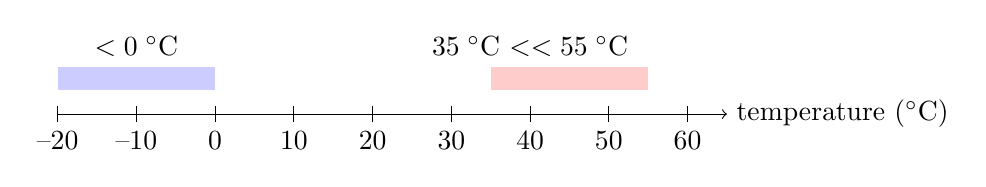
\begin{tikzpicture}
			% Draw temperature axis
			\draw[->] (0,0) -- (8.5,0) node[right] {temperature ($^\circ$C)};
			% Add tick marks and labels every 20 degrees from -20 to 100
			\foreach \x/\label in {0/--20, 1/--10, 2/0, 3/10, 4/20, 5/30, 6/40, 7/50, 8/60} {
			\draw (\x,0.1) -- (\x,-0.1);
			\node[below] at (\x,-0.1) {\label};
			}
			% Shade measurable set: Temperature < 0°C
			\fill[blue!20] (0,0.3) rectangle (2,0.6);
			\node[above] at (1,0.6) {$\outcome < 0\;^\circ$C};
			% Shade measurable set: 5°C < omega < 10°C
			\fill[red!20] (5.5,0.3) rectangle (7.5,0.6);
			\node[above] at (6,0.6) {$35\;^\circ$C $< \outcome < 55\;^\circ$C};
			\vspace*{10mm}
			\end{tikzpicture}
			\vspace*{10mm}
			\end{center}
			\caption{A \gls{samplespace} constituted by all possible temperature values $\outcome$ 
			that can occur at an \gls{fmi} station. Two measurable subsets of temperature 
			values, denoted by $\mathcal{A}^{(1)}$ and $\mathcal{A}^{(2)}$, are highlighted. For any 
			actual temperature value $\outcome$, it is possible to determine (via some equipment) 
			whether $\outcome \in \mathcal{A}^{(1)}$ and whether $\outcome \in \mathcal{A}^{(2)}$. 
			\label{fig_measurable_dict}} 
		\end{figure}
		In principle, measurable sets could be chosen freely (e.g., depending on the resolution of the 
		measuring equipment). However, it is often useful to impose certain completeness requirements 
		on the collection of measurable sets. For example, the \gls{samplespace} itself should be 
		measurable, and the union of two measurable sets should also be measurable. These completeness 
		requirements can be formalized via the concept of a \gls{sigmaalgebra} (or \gls{sigmafield}) 
		\cite{RudinBook}, \cite{BillingsleyProbMeasure}, \cite{durrett2010probability}. 
		A measurable space is a pair $\big(\featurespace,\eventspace\big)$ that consists of an arbitrary 
		set $\featurespace$ and a collection $\eventspace$ of measurable subsets of $\featurespace$ 
		that form a \gls{sigmaalgebra}. 
		\\
		See also: \gls{samplespace}, \gls{outcome}, \gls{sigmaalgebra}, \gls{probability}.},
	first={measurable},
	type=math, 
	text={measurable} 
}

\newglossaryentry{sigmaalgebra}
{name={$\sigma$-algebra}, 
sort={sigma-algebra},
	description={Consider a \gls{randomexperiment} with a \gls{samplespace} $\samplespace$. 
		A $\sigma$-algebra\index{$\sigma$-algebra} (or \gls{sigmafield}) $\sigmaalgebra$ 
		is a collection of subsets of $\samplespace$ with the following properties 
		\cite{RudinBook}, \cite{BillingsleyProbMeasure}, \cite{durrett2010probability}:
		\begin{itemize}
		 	\item The empty set $\emptyset$ and the entire \gls{samplespace} 
		 	$\samplespace$ belong to $\sigmaalgebra$, i.e., $\emptyset \in \sigmaalgebra$ and $\samplespace \in \sigmaalgebra$.
		 	\item If a set $\mathcal{A}$ belongs to $\sigmaalgebra$, then its complement 
		 	$\samplespace \setminus \mathcal{A}$ also belongs to $\sigmaalgebra$, i.e., 
		 	$\mathcal{A} \in \sigmaalgebra$ implies $\samplespace \setminus \mathcal{A} \in \sigmaalgebra$.
		 	\item If a \gls{countable} collection of sets $\mathcal{A}_1, \,\mathcal{A}_2, \,\ldots$ belongs 
			to $\sigmaalgebra$, 
		 	then their union also belongs to $\sigmaalgebra$, i.e.,
		 	$\mathcal{A}_1, \,\mathcal{A}_2, \,\ldots \in \sigmaalgebra$ implies 
		 	$\bigcup_{i=1}^{\infty} \mathcal{A}_i \in \sigmaalgebra$.	
		 \end{itemize}			 
		See also: \gls{samplespace}, \gls{rv}, \gls{probspace}.},
	first={$\sigma$-algebra},
	type=math, 
	text={$\sigma$-algebra} 
}

\newglossaryentry{sigmafield}
{name={$\sigma$-field}, 
sort={sigma-field},
	description={See \gls{sigmaalgebra}\index{$\sigma$-field}.}, 
	first={$\sigma$-field},
	type=math,
	text={$\sigma$-field} 
}

\newglossaryentry{injective}
{name={injective}, 
	description={A \gls{function} $f: \mathcal{U} \rightarrow \mathcal{V}$ is injective\index{injective} 
		if it maps distinct elements of its \gls{domain} to distinct elements 
		of its \gls{co-domain}, 
    		i.e., if $f(u_1) = f(u_2)$ implies $u_1 = u_2$ for all $u_1, u_2 \in \mathcal{U}$ 
        		\cite{HalmosSet}. 
    		Equivalently, no two different \gls{function} inputs are mapped to the same \gls{function} \gls{output}.
				\\
		See also: \gls{function}.},
	first={injective},
	type=math,
	text={injective} 
}

\newglossaryentry{typicalset}
{name={typical set}, 
	description={See \gls{pmf}\index{typical set}.}, 
 	first={typical set},
 	firstplural={typical sets},
 	type=math,
 	plural={typical sets},
 	text={typical set} 
}

\newglossaryentry{majmin}
{name={majorize-minimize (MM)}, 
	description={Consider an \gls{optproblem} $\min_{\weights \in \paramspace} f(\weights)$ with 
		some complicated (potentially non-\gls{convex} and \gls{nonsmooth}) \gls{objfunc}. 
		One important example of such an \gls{optproblem} is \gls{erm}, which is used to learn the 
		\glspl{modelparam} of a nonlinear \gls{model}. 
		An MM method is\index{majorize-minimize (MM)} an iterative \gls{optmethod} 
		that constructs a \gls{sequence} $\weights^{(1)},\,\weights^{(2)},\,\ldots \in \paramspace$ 
		of \glspl{modelparam} as follows \cite{Lange2016MM}, \cite{BishopBook}, \cite{Hunter01022004}
		(see also Fig. \ref{fig:majmin_dict}): 
		\begin{itemize} 
			\item During the $\iteridx$th \gls{iteration}, the \gls{objfunc} $f(\cdot)$ 
			 	is approximated by another \gls{function} $g\big(\cdot;\weights^{(\iteridx)}\big)$.
	             	  	This approximation must be an upper bound for (i.e., must majorize) the original
				\gls{objfunc}, i.e., $g\big(\weights;\weights^{(\iteridx)}\big) \geq f(\weights)$ 
			 	for all $\weights \in \paramspace$, and it must be tight for $\weights^{(\iteridx)}$, i.e., 
			 	$g\big(\weights^{(\iteridx)};\weights^{(\iteridx)}\big) = f\big(\weights^{(\iteridx)}\big)$.
			\item The new \glspl{modelparam}  $\weights^{(\iteridx+1)}$ are then obtained by 
				minimizing the approximation, i.e., 
				 $\weights^{(\iteridx+1)} \in \argmin_{\weights \in \paramspace}g\big(\weights;\weights^{(\iteridx)}\big)$. 
		\end{itemize} 
		\begin{figure}[H]
			 \centering
			 \begin{tikzpicture}[x=1.2cm,y=1cm]
				% --- parameters ---
				\def\xa{0}
				\def\xb{2*pi}
				\def\xo{3*pi/4}     % touch point: 1.5 * (pi/2) = 3pi/4
				\def\mL{0.4}        % left slope  (adjust to keep it above the sine)
				\def\mR{0.7}        % right slope (adjust to keep it above the sine)
				% horizontal axis
				\draw[->] (\xa-0.2,-2) -- (\xb+0.3,-2) node[right] {$\weights$};
				% sine over one period
				\draw[thick,samples=100,domain=\xa:\xb]
				plot (\x,{sin(\x r)}) node[pos=0.1,above left,black] {\small $f(\weights)$};
				% compute y0 = sin(w0)
				\pgfmathsetmacro\yxo{sin(\xo r)}
				% Anchors (numeric, no macros)
				% w0 = 3*pi/4 = 2.35619449
				% xL = 2.00619449, xR = 2.70619449
				% y0 = sin(w0) = 0.70710678
				% Left slope mL = cos(xL) = -0.42177145  (tangent => upper bound on [0, xL])
				% Right slope mR = 0.7  (rising; safely above the sine on [xR, 2*pi])
				\def\xL{2.70}
				\def\xR{3.80}
				\def\yO{0.70}
				% Left (tangent) segment: y = y0 + mL*(x - xL), mL = -0.42177145
				\draw[dashed,samples=2,domain=0:\xL]
				plot (\x,{\yO + (-0.7)*(\x - \xo)});
				% Flat touching segment
				\draw[dashed]
				(\xL,{\yO+(-0.7)*(\xL-\xo)}) -- (\xR,{\yO+(-0.7)*(\xL-\xo)});
				% Right rising segment: y = y0 + mR*(x - xR), mR = 0.7
				% draw the segment
				\draw[dashed,samples=2,domain=\xR:2*pi]
				plot (\x,{\yO+(-0.7)*(\xL-\xo) + (0.7)*(\x - \xR)});
				% compute a point 65% along the x-range [\xR, 2*pi]
				\pgfmathparse{\xR + 0.65*(2*pi - \xR)} \let\xmid\pgfmathresult
				\pgfmathparse{\yO + 0.7*(\xmid - \xR)} \let\ymid\pgfmathresult
				% label at that point
				\node[right,black] at (\xmid,\ymid) {$g\big( \weights; \weights^{(\iteridx)} \big)$};
				% Touch marker at w0
				\fill[red] (2.35619449,0.70710678) circle (1.2pt);
				% --- vertical ruler marking w0 ---
				\draw[densely dotted,gray] (\xo,-2) -- (\xo,\yO);
				% \draw[gray] (\xo,0) -- ++(0,-2.06);
				\node[below] at (\xo,-2) {$\weights^{(\iteridx)}$};
			\end{tikzpicture}
		\caption{The construction of \glspl{modelparam} based on the iterative MM method.}
			\label{fig:majmin_dict}
		\end{figure}
		Similar to \glspl{gdmethod}, the MM principle is also based on approximating an 
		\gls{objfunc} locally, around the current \glspl{modelparam}, and then optimizing 
		this approximation to obtain new \glspl{modelparam}. However, the construction 
		of local approximations is very different. While \glspl{gdmethod} use linear \glspl{function} 
		for these approximations, MM methods can use nonlinear \glspl{function} as long as 
		they are upper bounds for the original \gls{objfunc}. 
			 \\ 
		See also: \gls{gdmethod}, \gls{em}.},
	first={majorize–minimize (MM)},
	type=math, 
	text={MM}
}

\newglossaryentry{markovsinequality}
{name={Markov's inequality},
	description={Consider a real-valued nonnegative \gls{rv} $x$ for which 
		the \gls{expectation} $\expect\{ x\}$ exists. \index{Markov's inequality} 
	 	Markov's inequality provides an upper bound on the \gls{probability} 
	 	$\prob{x\geq a}$ that $x$ exceeds a given positive threshold $a>0$.  
	 	In particular,          
	 	\begin{equation}
            		\nonumber
			\prob{x \geq a} \leq \frac{\expect \{ x\}}{a} \qquad \mbox{ holds for any } a > 0. 
            		%\label{eq:markovsinequality_dict}
    		\end{equation}
    		This inequality can be verified by noting that $\prob{x \geq a}$ is the 
		\gls{expectation} $\expect\{g(x)\}$ with the \gls{function} 
	 	$$g: \mathbb{R} \rightarrow \mathbb{R}: x' \mapsto \indicatorfunc{\{x \geq a\}}(x').$$ 
	 	As illustrated in Fig. \ref{fig:markovsinequality_dict}, for any positive $a>0$, 
	 	$$ g(x') \leq x'/a \mbox{ for all } x' \in \mathbb{R}.$$ 
	 	This implies Markov's inequality via the monotonicity property 
	 	of the \gls{LebesgueIntegral} \cite[p. 50]{folland1999real}. 
    		\begin{figure}[H]
			\centering
			\begin{tikzpicture}[scale=1, x=0.8cm, y=0.8cm]
			% -------- parameters ----------
			\def\a{3.24}      % threshold a
			\def\xmax{10}     % x-axis max
			\def\m{0.02}      % slope of the linear function y = m(x-a)+1
			% -------- pdf function p(x) (same as your expression) ----------
			% p(x) = (1/(3*sqrt(2*pi))) * x^(1.5) * exp(-x/2)
			\draw[-{Latex}] (0,0) -- (\xmax+1,0) node[below right] {$x'$};
			%\draw[-{Latex}] (0,0) -- (0,3.1) node[left] {$\pdf{x}{x'}$};
                		\draw[-{Latex}] (0,0) -- (0,3.1)  node[left, text=blue!70!black] {$\pdf{x}{x'}$};
			% Fill under the pdf (optional aesthetics)
			\fill[blue!15, opacity=0.3]
			plot[samples=400, domain=0:\xmax, smooth]
			(\x,{ (6/sqrt(2*pi)) * (\x)^(1.5) * exp(-\x/2) }) -- (\xmax,0) -- (0,0) -- cycle;
			% PDF curve
			\draw[blue!70!black, very thick, samples=400, domain=0:\xmax, smooth]
			plot (\x,{ (6/(sqrt(2*pi))) * (\x)^(1.5) * exp(-\x/2) })
			node[pos=0.9, above right, xshift=2pt] {};
			% Vertical guide at x=a
			\draw[dashed, gray] (\a,0) -- (\a,1.05);
			\node[below] at (\a,0) {$a$};
			\node[above] at (1*\a,3) {$\prob{x \geq a} \leq \frac{\expect \{ x\}}{a}$}; 
			\node[below] at (0,0) {$0$};
			% -------- indicator 1{x >= a} ----------
			% 0 for x<a with open circle at (a,0)
			\draw[green!60!black, ultra thick] (0,0) -- (\a,0);
			\filldraw[white, draw=green!60!black, line width=0.8pt] (\a,0) circle (2pt);
			% 1 for x>=a with closed circle at (a,1)
			\draw[green!60!black, ultra thick] (\a,1) -- (\xmax,1)
			node[pos=0.9, above, yshift=2pt] {$\indicatorfunc{\{x \ge a\}}(x')$};
			\filldraw[green!60!black] (\a,1) circle (2pt);
			% -------- linear curve through (a,1): y = m(x-a)+1 ----------
			\draw[red!70, very thick, samples=2, domain=0:\xmax]
			plot (\x,{ \x*(1/\a) }); 
			\node[align=right,red!70,yshift=20pt] at ({2.5*\a+0.2},{2.5}) {$f(x') = x'/a$};  
			% Axis marker for y=1
			\draw (0,1) -- ++(-0.12,0) node[left] {$1$};
			\end{tikzpicture}
            	\caption{The \gls{expectation} $\expect\{x\}$ and the \gls{probability} $\prob{x \geq a}$ 
			of a nonnegative \gls{rv} $x$ with a \gls{pdf} $\pdf{x}{\cdot}$           
                		%a \gls{probdist} $\probdist^{(x)}$ 
			can be obtained via \glspl{LebesgueIntegral} of 
			$f(x') = x'/a$ and $g(x') = \indicatorfunc{\{x \geq a\}}(x')$, respectively.}
            		\label{fig:markovsinequality_dict}
        		\end{figure} 
		See also: \gls{expectation}, \gls{probability}, \gls{concentrationinequ}.},
	first={Markov's inequality},
	type=math, 
    	text={Markov's inequality}  
}

\newglossaryentry{chebyshevsinequality}
{name={Chebyshev's inequality},
	description={Consider a real-valued \gls{rv} $x$ for which 
		the second moment $\expect\{ x^{2} \}$ exists (and is finite). 
 	 	The existence of the second moment implies the existence 
 	 	of a finite \gls{expectation} $\mu \defeq \expect\{ x\}$ and a finite 
 	 	\gls{variance} $\sigma^{2}\!\defeq\!\expect \big\{ \big( x\!-\!\mu \big)^{2} \big\}$ \cite[Proposition 6.12]{folland1999real}. 
 	 	Chebyshev's inequality\index{Chebyshev's inequality} refers 
 	 	to the following upper bound on the \gls{probability} that $x$ 
 	 	deviates from $\mu$ by more than a given threshold $\eta$ 
 	 	\cite[Ch. 4]{FellerBook}. 
 	 	In particular,   
 		\begin{equation}
           		\nonumber
			\prob{\big|x - \mu \big| \geq \eta } \leq \frac{\sigma^2}{\eta^2} \qquad \mbox{ for some } \eta > 0.
            		%\label{eq:chebyshevsinequality_dict}
     		\end{equation}
 		This upper bound can be obtained by applying \gls{markovsinequality} to 
 		the new \gls{rv} $\tilde{x}\!\defeq\! \big(x\!-\!\mu \big)^2$. 
  		\begin{figure}[H]
   			\centering
			\begin{tikzpicture}
     			\begin{axis}[
      			width=9cm, height=4.2cm,
      			samples=300,
      			axis lines=left,
	  		ylabel={$\pdf{x}{x'}$},
      			xlabel={$x'$},
      			x label style={at={(axis description cs:1,0)}, anchor=west},
	  		ylabel style={rotate=270,anchor=south,at={(axis description cs:0,1.02)}},
      			xtick={-1.5,0,1.5},
      			xticklabels={$-\eta$,$\mu$,$\eta$},
      			ytick=\empty,
      			ymin=0, ymax=0.45,
      			domain=-4:4,
      			clip=false
    			]
      			% pdf (centered at mu; here shown as standard normal in x - mu coordinates)
      			\addplot[name path=pdf, black, very thick] {exp(-0.5*x^2)/sqrt(2*pi)};
      			\addplot[name path=axis, draw=none] {0};
      			% shaded tails: |X - mu| >= t with t = 1.5
      			\addplot[red!70, opacity=0.25] fill between[of=pdf and axis, soft clip={domain=1.5:4}];
      			\addplot[red!70, opacity=0.25] fill between[of=pdf and axis, soft clip={domain=-4:-1.5}];
      			% guide lines at mu and ±t
      			\draw[densely dashed] (axis cs:0,0) -- (axis cs:0,0.42);
      			\draw[dashed] (axis cs:1.5,0) -- (axis cs:1.5,{exp(-0.5*1.5^2)/sqrt(2*pi)});
      			\draw[dashed] (axis cs:-1.5,0) -- (axis cs:-1.5,{exp(-0.5*1.5^2)/sqrt(2*pi)});
      			% label for the shaded area
   			%   \node[anchor=west] at (axis description cs:0.72,0.82) {$\prob{|x-\mu|\ge \eta}$};
    			\end{axis}
  			\end{tikzpicture}
  		\caption{Chebyshev's inquality provides an upper bound on 
              		the tail \gls{probability} $\prob{|x-\mu|\ge \eta}$ (i.e., shaded area) of
			a real-valued \gls{rv} $x$ with a finite second moment.\label{fig:chebyshev_minimal_dict}} 
		\end{figure}
     		See also: \gls{expectation}, \gls{markovsinequality}, \gls{concentrationinequ}.},
    	first={Chebyshev's inequality},
	type=math, 
     	text={Chebyshev's inequality}  
}

\newglossaryentry{hoeffdingsinequality}
{name={Hoeffding's inequality},
	description={\index{Hoeffding's inequality} Hoeffding's inequality \cite{Hoeffding1963} is a fundamental \gls{concentrationinequ} 
		that provides an upper bound on the \gls{probability} that a sum (or average) of independent, bounded \glspl{rv} 
		deviates from its \gls{mean} by more than some threshold. 
     		Let $x_1,\,\dots,\,x_n$ be independent real-valued \glspl{rv} $x_i$ taking values in $[a_i,b_i] \subset \mathbb{R}$, 
		and $S_n \defeq \sum_{i=1}^n x_i$ and $\expect\{S_n\} = \sum_{i=1}^n \expect\{x_i\}$. 
		Then, Hoeffding's inequality \cite[Th. 2.2.6]{vershynin2018high} states that
        		\begin{equation}
                		\nonumber
			\prob{ |S_n - \expect\{S_n\}| \geq t } 
            		\leq 2 \exp \left( -\frac{2 t^2}{\sum\limits_{i=1}^n (b_i - a_i)^2} \right) \qquad \forall t > 0.
            		%\label{eq:hoeffding_sum}
        		\end{equation}
    		Hoeffding's inequality typically provides sharper bounds than \gls{chebyshevsinequality}, 
		but it is more restrictive by assuming bounded \glspl{rv}.
    		In the context of \gls{ml}, this result is useful for deriving guarantees for \gls{erm}  and in the context of \gls{mab}. 
		 \\
    		See also: \gls{concentrationinequ}, \gls{probability}, \gls{rv}, \gls{chebyshevsinequality}, \gls{expectation}, \gls{probspace}, \gls{markovsinequality}.},
    	first={Hoeffding's inequality},
	type=math, 
    	text={Hoeffding's inequality}  
}

\newglossaryentry{rgg}
{name={random geometric graph (RGG)},
	description={An RGG\index{random geometric graph (RGG)} is a \gls{probmodel} for \glspl{graph} 
		built from nodes randomly placed in a \gls{metricspace}. Given a \gls{metricspace}, the RGG is characterized by 
		the number of nodes, the connection radius, and the \gls{probdist} describing the node placement. 
    		More precisely, for a node set $\nodeidx=1, \,\ldots, \,\nrnodes$, each node $\nodeidx$ is assigned to a random position 
		$\featurevec^{(\nodeidx)} \in \featurespace$, typically as \glspl{realization} of \gls{iid} \glspl{rv} taking values in a set $\featurespace$. 
		Together with a \gls{metric}, this forms a \gls{metricspace}, often with the \gls{metric} induced by a \gls{norm}. 
		A specific \gls{realization} of an RGG contains an edge $\edge{\nodeidx}{\nodeidx'}$ if and only if the distance between the nodes 
		with respect to the \gls{metric} is smaller than some threshold, i.e., when $\metric{\featurevec^{(\nodeidx)}}{\featurevec^{(\nodeidx')}}\leq r$ 
		for some threshold $r>0$, as illustrated in Fig. \ref{fig:rgg}.
         	\begin{figure}[H]
    			\centering
    			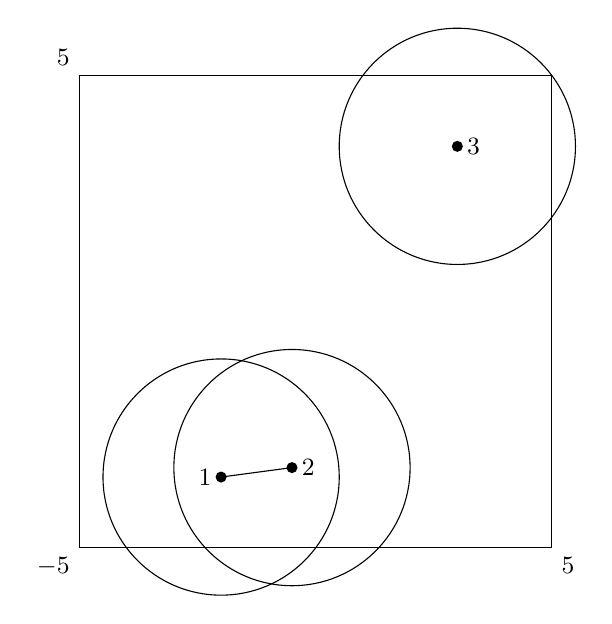
\begin{tikzpicture}[x=0.6cm,y=0.6cm]
        				\draw (-5,-5) rectangle (5,5);
        				% Corner labels outside the rectangle
        				\node[below left] at (-5,-5) {\small $-5$};
        				\node[above left]  at (-5, 5) {\small $5$};
        				\node[below right] at ( 5,-5) {\small $5$};
        				% Bottom two points (nodes 1 and 2) within each other's circle of radius 2.5
        				\fill (-2.0,-3.5) circle (2pt);
        				\draw (-2.0,-3.5) circle (2.5);
        				\node[anchor=east] at (-2.0,-3.5) {\small 1};
        				\fill (-0.5,-3.3) circle (2pt);
        				\draw (-0.5,-3.3) circle (2.5);
        				\node[anchor=west] at (-0.5,-3.3) {\small 2};
        				\draw (-2.0,-3.5) -- (-0.5,-3.3);
        				% Top point (node 3) outside the bottom circles
        				\fill (3.0,3.5) circle (2pt);
        				\draw (3.0,3.5) circle (2.5);
        				\node[anchor=west] at (3.0,3.5) {\small 3};
    			\end{tikzpicture}
   		\caption{Illustration of an RGG with $ \featurespace = [-5,5]\times[-5,5] \subset \mathbb{R}^2$ and radius $r=2.5$ 
			(with respect to the \gls{eucliddist}), where nodes 1 and 2 (corresponding to $(-2.0, -3.5)^T$ and $(-0.5, -3.3)^T$, 
			within radius $r=2.5$) are connected, while node 3 (corresponding to $(3.0, 3.5)^T$) has no other node within that distance.}
    			\label{fig:rgg}
    		\end{figure}
        		See also: \gls{graph}, \gls{sbm}, \gls{ergraph}.},
    	first={random geometric graph (RGG)},
	type=math, 
    	text={RGG}
}

\newglossaryentry{banachfixedpoint}
{name={Banach's fixed-point theorem},
	description={Banach's fixed-point theorem\index{Banach's fixed-point 
		theorem} (also referred to as the contraction 
		principle \cite[Th. 9.23]{RudinBookPrinciplesMatheAnalysis}) 
		states that every \gls{contractop} $\fixedpointop$ on a complete 
		\gls{metricspace} has a unique fixed point. Formally, 
		let $(\featurespace,\metric{\cdot}{\cdot})$ be a non-empty complete 
		\gls{metricspace} and let $\fixedpointop:\featurespace\to\featurespace$ satisfy
    		\[
    		\metric{\fixedpointop \featurevec}{\fixedpointop \featurevec'} \leq \kappa \cdot \metric{\featurevec}{\featurevec'} \qquad \forall \featurevec,\featurevec'\in\featurespace
    		\]
    		for some constant $\kappa \in [0,1)$. Then, $\fixedpointop$ has a unique fixed 
		point, i.e., there exists a unique $\featurevec^\star\in\featurespace$ with 
		$\fixedpointop \featurevec^\star =\featurevec^\star$, which can be computed by a 
		\gls{fixedpointiter}.
    		\begin{figure}[H]
    			\centering
    			\begin{tikzpicture}[>=Latex, font=\small]
    			\tikzset{space/.style={draw, thick, circle, minimum size=4.0cm},pt/.style={circle, inner sep=1.5pt, draw, fill=black},maparrow/.style={->, very thick},link/.style={->, thick},distline/.style={dashed, thick}}
    			\def\dx{6.5}
    			\node[space,label=above:{$\featurespace$}] (XL) at (0,0) {};
    			\node[space,label=above:{$\featurespace$}] (XR) at (\dx,0) {};
    			\draw[maparrow] (XL.east) -- node[above=2pt] {$\fixedpointop$} (XR.west);
    			\coordinate (x1) at (-0.8,0.9);
    			\coordinate (x2) at (0.9,0.5);
    			\node[pt,label=above left:{$\featurevec$}] at (x1) {};
    			\node[pt,label=right:{$\featurevec'$}] at (x2) {};
    			\coordinate (fx1) at (\dx-0.3,0.5);
    			\coordinate (fx2) at (\dx+0.6,0.5);
    			\node[pt] (FX1) at (fx1) {};
    			\node[pt] (FX2) at (fx2) {};
    			\node[anchor=east] at ($(FX1.west)+(-6pt,-2pt)$) {$\fixedpointop \featurevec$};
    			\node[anchor=west] at ($(FX2.east)+(6pt,-2pt)$) {$\fixedpointop \featurevec'$};
   			% \draw[distline] (x1) -- (x2) node[midway, above=6pt, sloped] {$\metric{\fixedpointop \featurevec}{\fixedpointop \featurevec'}$};
   			% \draw[distline] (fx1) -- (fx2) node[midway, above=6pt, sloped] {$\metric{\featurevec}{\featurevec'}$};
    			\coordinate (xsL) at (0,-0.9);
    			\coordinate (xsR) at (\dx,-0.9);
    			\node[pt,label=below:{$\featurevec^\star$}] at (xsL) {};
    			\node[pt,label=below:{$\fixedpointop \featurevec^\star=\featurevec^\star$}] at (xsR) {};
    			\end{tikzpicture}
   	 	\caption{A \gls{contractop} $\fixedpointop:\featurespace\to\featurespace$  
	  		has a unique fixed point $\featurevec^\star$ with $\fixedpointop \featurevec^\star=\featurevec^\star$.}
    			\label{fig:banach_dict}
    		\end{figure}
    		See also: \gls{contractop}, \gls{metricspace}, \gls{fixedpointiter}, \gls{sequence}, \gls{cauchysequence}.},
    	first={Banach's fixed-point theorem},
	text={Banach's fixed-point theorem},
    	type=math
}

\newglossaryentry{diagonalizable}
{name={diagonalizable},
	description={A square \gls{matrix} $\mA \in \mathbb{C}^{\nrfeatures \times \nrfeatures}$ 
		is called diagonalizable\index{diagonalizable} if it is similar  
 		to a diagonal \gls{matrix} \cite{HornMatAnalysis}, \cite{Axler2025}. 
 		Formally, $\mA$ is diagonalizable if there exists an invertible \gls{matrix} 
		$\mP \in \mathbb{C}^{\nrfeatures \times \nrfeatures}$ such that 
  		\[
  			\mA = \mP \mD \mP^{-1}
  		\]
		where $\mD \in \mathbb{C}^{\nrfeatures \times \nrfeatures}$ is a 
 		diagonal \gls{matrix} whose main diagonal entries are the \glspl{eigenvalue} 
 		of $\mA$. A \gls{matrix} $\mA \in \mathbb{R}^{\nrfeatures \times \nrfeatures}$ 
 		is diagonalizable if and only if it has $\nrfeatures$ linearly independent 
 		\glspl{eigenvector} \cite{HornMatAnalysis}. 
 		\\	
 		See also: \gls{matrix}, \gls{eigenvalue}, \gls{evd}.},
 	first={diagonalizable},
 	type=math,
 	text={diagonalizable}
}

\newglossaryentry{schurdecomp}
{name={Schur decomposition},
 description={Every square \gls{matrix} $\mA \in \mathbb{C}^{\nrfeatures \times \nrfeatures}$ 
              admits a Schur decomposition\index{Schur decomposition} \cite[Thm. 7.1.3]{GolubVanLoanBook}
			\[\mA = \mU \mT \mU^{H}. 
			\]
			Here, $\mU \in \mathbb{C}^{\nrfeatures \times \nrfeatures}$ is a unitary 
			matrix (i.e., $\mU^{H}\mU = \mI$) and $\mT$ is upper triangular 
			with the \glspl{eigenvalue} of $\mA$ on its diagonal.
			Carefully note that the Schur decomposition exists also 
			for a \gls{matrix} $\mA$ that is not \gls{diagonalizable}, 
			\begin{figure} 
				\[
				\big(\mU^{(1)}\big)^{H} \mA \mU^{(1)}
				=
				\begin{pmatrix}
				\big(\vx^{(1)}\big)^{H} \\
				\big(\mX^{(2)}\big)^{H}
				\end{pmatrix}
				\mA
				\begin{pmatrix}
				\vx^{(1)} & \mX^{(2)}
				\end{pmatrix}
				=
				\begin{pmatrix}
				\eigval{1} & \vb^{H} \\
				0 & \mA^{(1)}
				\end{pmatrix},
				\]
				\caption{The first step in the construction of the Schur decomposition.
					Every \gls{matrix} $\mA \in \mathbb{C}^{n\times n}$ has at least one 
				     \gls{eigenvalue} $\eigval{1}$ with unit-norm \gls{eigenvector} 
					 $\vx^{(1)}$, $\mA \vx^{(1)} = \eigval{1} \vx^{(1)}$. This 
					 \gls{eigenvector} allows to decompose $\mA$ as depicted. Here, 
					 we extended $\vx^{(1)}$ to an orthonormal basis
					$\mQ^{(1)} = \big( \vx^{(1)} \,\big|\, \mX^{(2)} \big)$
					and used $\vb^{H} := \big(\vx^{(1)}\big)^{H} \mA \mX^{(2)}$ and 
					$\mA^{(1)} := \big(\mX^{(2)}\big)^{H} \mA \mX^{(2)}$.
			 		Applying the same construction recursively to $\mA^{(1)}$ yields the 
				     Schur decomposition.}
			\end{figure}
			\\
 		See also: \gls{evd}, \gls{eigenvalue}, \gls{matrix}.},
	first={Schur decomposition},
	type=math,
	text={Schur decomposition}
}

\newglossaryentry{unitary}
{name={unitary (matrix)},
 description={A square \gls{matrix} $\mU \in \mathbb{C}^{\nrfeatures \times \nrfeatures}$ 
			  is called unitary\index{unitary matrix} if its conjugate 
			  transpose (Hermitian transpose) $\mU^{H}$ is also its inverse, i.e., if 
 		\[
 			\mU^{H} \mU = \mU \mU^{H} = \mI.
 		\]
 		Equivalently, the columns (and rows) of a unitary \gls{matrix} form an 
		orthonormal basis of $\mathbb{C}^{\nrfeatures}$ with respect to the standard 
		inner product\cite{HornMatAnalysis,Axler2025}. 
 		\\
 		See also: \gls{matrix}.},
 	first={unitary},
 	type=math,
 	text={unitary}
}

\newglossaryentry{innerproduct}
{name={inner product},
 description={Consider a \gls{vectorspace} $\featurespace$ over the 
              field $\mathbb{F}$, where $\mathbb{F}$ is either the field of 
			  real numbers $\mathbb{R}$ or the field of complex numbers $\mathbb{C}$. 
	          An inner product\index{inner product} in $\featurespace$ is 
			  a \gls{function} 
 			 \[
 				\innerprod{\cdot}{\cdot}: \featurespace \times \featurespace \to \mathbb{F},
 			 \]
 			 that satisfies the following properties for all 
			 $\featurevec, \featurevec', \featurevec'' \in \featurespace$ 
				and all scalars $\alpha \in \mathbb{F}$ \cite{Axler2025}:
 			\begin{itemize}
 				\item[(i)] Conjugate symmetry: $\innerprod{\featurevec}{\featurevec'} = \overline{\innerprod{\featurevec'}{\featurevec}}$,
 				\item[(ii)] Linearity in the first argument: $\innerprod{\alpha \featurevec + \featurevec''}{\featurevec'} = \alpha \innerprod{\featurevec}{\featurevec'} + \innerprod{\featurevec''}{\featurevec'}$,
 				\item[(iii)] Positive-definiteness: $\innerprod{\featurevec}{\featurevec} \geq 0$, with equality if and only if $\featurevec = \mathbf{0}$.
 			\end{itemize}
 			The pair $(\featurespace, \innerprod{\cdot}{\cdot})$ is called an inner product space. 
			Each inner product induces a \gls{norm} via 
			$\norm{\featurevec} \defeq \sqrt{\innerprod{\featurevec}{\featurevec}}$ for all 
			$\featurevec \in \featurespace$, which in turn induces a \gls{metric} via 
			$\metric{\featurevec}{\featurevec'} \defeq \norm{\featurevec - \featurevec'}$
			for all $\featurevec, \featurevec' \in \featurespace$.
 		\\
 		See also: \gls{vector}, \gls{norm}, \gls{metricspace}.},
 	first={inner product},
 	type=math,
 	text={inner product}
}

\newglossaryentry{trace}
{name={trace (matrix)},
  description={The\index{trace} trace $\tr{\mA}$ of a square \gls{matrix} 
         	   $\mA \in \mathbb{R}^{\nrfeatures \times \nrfeatures}$ is the 
			   sum of its diagonal entries \cite{StrangLinAlg2016}. 
		 	   Formally, it is the \gls{linearmap} 
		 		$$\tr{\cdot}: \mathbb{R}^{\nrfeatures \times \nrfeatures} 
		 			\rightarrow \mathbb{R}: \mA \mapsto \sum_{\featureidx=1}^{\nrfeatures} A_{\featureidx,\featureidx}.$$     
    	 		It satisfies the cyclic property $\tr{\mA\mB}=\tr{\mB\mA}$, for any \glspl{matrix} 
    	 		$\mA,\mB \in \mathbb{R}^{\nrfeatures \times \nrfeatures}$ \cite[p. 301]{Axler2025}.
				\begin{figure}
					\begin{center}
				\begin{tikzpicture}[font=\small, every node/.style={inner sep=1pt}]
					% Matrix entries, manually placed
				\node (a11) at (0,0)   {$A_{1,1}$};
				\node (a12) at (1,0)   {$A_{1,2}$};
				\node (a13) at (2,0)   {$A_{1,3}$};
				\node (a21) at (0,-1)  {$A_{2,1}$};
				\node (a22) at (1,-1)  {$A_{2,2}$};
				\node (a23) at (2,-1)  {$A_{2,3}$};
				\node (a31) at (0,-2)  {$A_{3,1}$};
				\node (a32) at (1,-2)  {$A_{3,2}$};
				\node (a33) at (2,-2)  {$A_{3,3}$};
				% Very light bounding box (optional)
				\draw[black] (-0.4,0.4) rectangle (2.4,-2.4);
				% Tight ellipse around diagonal entries
				\coordinate (C) at ($(a11)!0.5!(a33)$);
				\draw[thick] (C) ellipse [x radius=2.1cm, y radius=0.35cm,rotate=-45];
				\end{tikzpicture}
				\end{center}
				\caption{The trace $\tr{\mA}$ of a $3 \times 3$ matrix $\mA \in \mathbb{R}^{3\times 3}$ is 
				the sum of three main diagonal entries $A_{1,1}, A_{2,2}, A_{3,3}$.}
				 \end{figure}
				Furthermore, if $\mA$ has \glspl{eigenvalue} $\eigval{1},\ldots,\eigval{\nrfeatures}$ 
				(each repeated according to its algebraic multiplicity), then
				\[\tr{\mA} = \sum_{\featureidx=1}^{\nrfeatures} \eigval{\featureidx}.
				\]
				This identity follows from the invariance of the trace under similarity 
				transformations \cite[Ch.~10]{Axler2025}.\\
    			See also: \gls{eigenvalue}, \gls{matrix}.},
    first={trace},
    type=math,
    text={trace}
}
 
\newglossaryentry{stddev}
{name={standard deviation},
	description={The\index{standard deviation} standard deviation of a 
               	real-valued \gls{rv} $\feature$ is defined as the square 
		root of its \gls{variance}, i.e., 
		$\sqrt{\expect\big\{ \big( \feature - \expect\{\feature \} \big)^{2} \big\}}$. 
		\\
    		See also: \gls{rv}, \gls{variance}, \gls{expectation}.},
    first={standard deviation},
    type=math,
    text={standard deviation}
}

\newglossaryentry{sequence}
{name={sequence},
	description={A sequence\index{sequence} is an ordered collection 
		of values from a set $\mathcal{A}$. For example, a sequence of 
	   	values from the set $\mathcal{A} = \{ \star, \otimes \}$ could be 
	   	$$ a = \big( \star, \,\otimes, \,\star, \,\star, \,\otimes, \,\ldots \big). $$
	   	Formally, a sequence $a$ is a \gls{function} \cite{RudinBookPrinciplesMatheAnalysis} 
        		\[
            	a: \mathbb{N} \rightarrow \mathcal{A}: \sampleidx \mapsto a_\sampleidx.
        		\]        
		We denote a sequence by $\big( a_{\sampleidx} \big)_{\sampleidx \in \mathbb{N}}$ 
		or $\big( a^{(\sampleidx)} \big)_{\sampleidx \in \mathbb{N}}$. Sometimes we also 
		use the notation $\big\{ a^{(\sampleidx)} \big\}_{\sampleidx \in \mathbb{N}}$. 
        		Note that the same value $a \in \mathcal{A}$ can appear multiple times 
		in the sequence at different positions $\sampleidx$. 		
        		Sequences are fundamental for the study of \gls{ml} methods, 
        		for instance when describing successive iterates  
        		$\{\weights^{(\iteridx)}\}_{\iteridx \in \mathbb{N}}$ of an iterative 
		\gls{algorithm}. We can also use a sequence to represent an infinite 
		\gls{dataset} 
		$$\dataset = \big\{ \pair{\featurevec^{(1)}}{\truelabel^{(1)}},\,\pair{\featurevec^{(2)}}{\truelabel^{(2)}},\,\ldots \big\}.$$ 
		See also: \gls{function}, \gls{dataset}. }, 
	first={sequence},
	text={sequence},
	type=math, 
	firstplural={sequences},
	plural={sequences}
}

\newglossaryentry{convergence}
{name={convergence},
	description={Consider a \gls{sequence}\index{convergence} $\big( a_{\sampleidx} \big)_{\sampleidx \in \mathbb{N}}$ 
		with numeric values $a_{\sampleidx} \in \mathbb{R}$. This \gls{sequence} 
       	 	is said to converge to a value $a^\star$ if the values $a_{\sampleidx}$ become 
		arbitrarily close to $a^\star$ for sufficiently large indices $\sampleidx$. 
        		Mathematically speaking, the \gls{sequence} converges to $a^\star$ if 
		\cite{RudinBook}, \cite{RudinBookPrinciplesMatheAnalysis}
        		\[
           	\forall \epsilon > 0, \; \exists N \in \mathbb{N} : \sampleidx > N \Rightarrow |a_{\sampleidx} - a^\star| < \epsilon.
        		\]
		We denote the convergence of a \gls{sequence} to $a^\star$ 
		by 
		\[
			\lim_{\sampleidx \to \infty} a_{\sampleidx} = a^\star.
		\]
		\begin{figure}[H] 
			\centering
			\begin{tikzpicture}[x=1.2cm, y=2cm, >=stealth]
			% Axes
			\draw[->] (0.5,0) -- (6.5,0) node[right] {$\sampleidx$};
			\draw[->] (0.5,0) -- (0.5,1.6) node[above] {$a_\sampleidx$};
			% Epsilon neighbourhood (ε = 0.1)
  			\def\eps{0.3}
  			\fill[gray!30, opacity=0.4] (0, {1-\eps}) rectangle (6.3, {1+\eps});
  			\draw[dotted] (0,{1+\eps}) -- (6.3,{1+\eps}) node[right] {$1+\varepsilon$};
  			\draw[dotted] (0,{1-\eps}) -- (6.3,{1-\eps}) node[right] {$1-\varepsilon$};
			% Limit line at 1
			\draw[dashed] (0,1) -- (6.3,1) node[right] {$\lim_{\sampleidx \to \infty} a_\sampleidx = 1$};
			% Sequence points (e.g. a_t = 1 - 0.6^t)
			\foreach \t in {1,...,6} {
			\pgfmathsetmacro{\at}{1 - 0.6^(\t)}
			\fill (\t,\at) circle (2pt);
			}
			% Tick marks at t = 1, 2, 3
 		     	\foreach \t in {1,2,3} {
    		    	\draw (\t,0.02) -- (\t,-0.02) node[below] {$\t$};
  		    	}
			% Indicate N (first index within ε-band)
  			\def\N{3}
  			\draw[densely dashed, thick, red] (\N,0) -- (\N,1.7);
  			\node[above] at (\N,1.7) {$N$};
			\end{tikzpicture}
		\caption{A real-valued sequence $\big( a_{\sampleidx} \big)_{\sampleidx \in \mathbb{N}}$ 
			converging to the limit $a^\star = 1$.\label{fig:convergence_dict}}
		\end{figure} 
		The concept of convergence of a real-valued \gls{sequence} 
		(where $\mathcal{A}=\mathbb{R}$) extends naturally to a \gls{sequence} 
		in an arbitrary \gls{metricspace} $\mathcal{A}$. Indeed, we just need to 
		replace the absolute difference $|a_{\sampleidx} - a^\star|$ 
		by the \gls{metric} $\metric{a_{\sampleidx}}{a^\star}$. 
		Note that a \gls{sequence} can only converge if it is a 
		\gls{cauchysequence} \cite{RudinBookPrinciplesMatheAnalysis}. 
		However, not every \gls{cauchysequence} is converging unless 
		the underlying \gls{metricspace} is complete.   
		\\ 
		See also: \gls{sequence}, \gls{metricspace}, \gls{cauchysequence}.},
	first={convergence},
	type=math,
	text={convergence}, 
}

\newglossaryentry{johnsonlindenstrausslemma}
{name={Johnson--Lindenstrauss lemma (JL lemma)},
	description={The\index{Johnson--Lindenstrauss lemma (JL lemma)} JL lemma describes conditions for 
  		the existence of a \gls{featuremap} $\featuremapvec: \mathbb{R}^{\nrfeatures} \to \mathbb{R}^{\nrfeatures'}$ 
  		with $\nrfeatures' \ll \nrfeatures$ such that the pairwise \gls{eucliddist} 
  		between \glspl{featurevec} of a finite \gls{dataset} is approximately preserved 
  		\cite{vershynin2018high}, \cite{JMLR:v19:18-264}, \cite{johnson1984extensions}. 
  		Consider a \gls{dataset} $\dataset = \big\{\featurevec^{(1)}, \,\dots, \,\featurevec^{(\samplesize)} \big\}$ 
  		with \glspl{datapoint} characterized by \glspl{featurevec} in $\mathbb{R}^{\nrfeatures}$. 
  		Then, for any $\nrfeatures'$ that satisfies
		\[
	  	\nrfeatures' \ge \frac{4 \ln(\samplesize)}{\varepsilon^2/2 - \varepsilon^3/3} \mbox{ for some } 0 < \varepsilon < 1
		\]  
   		there is a \gls{featuremap} $\featuremapvec$ such that \cite{ProofJLlemma}
  		\begin{equation} 
 			\label{equ_def_approx_norm_JL_lemma_dict}
 			(1\!-\!\varepsilon)\normgeneric{\featurevec^{(\sampleidx)}\!-\!\featurevec^{(\sampleidx')}}{2}  
 			\!\le\!\normgeneric{\featuremapvec\big(\featurevec^{(\sampleidx)}\big)\!-\!\featuremapvec\big(\featurevec^{(\sampleidx')}\big)}{2} 
			\!\le\!(1\!+\!\varepsilon)\normgeneric{\featurevec^{(\sampleidx)}\!-\!\featurevec^{(\sampleidx')}}{2}
 		\end{equation}
		for all $\featurevec^{(\sampleidx)}, \featurevec^{(\sampleidx')} \in \dataset$. 
		\begin{figure}[H]
			\centering
			\begin{tikzpicture}
			% ---------- Original space: R^d ----------
			\begin{scope}
				% Points
				\coordinate (x1) at (0.5,-0.6);   % anchor
				\coordinate (x2) at (2.0,0.9);    % farther from x1 (long)
				\coordinate (x3) at (1.1,0.3);    % closer to x1 (short)
				\foreach \p in {x1,x2,x3} \fill (\p) circle (1.7pt);
				% Labels
				\node[below left]  at (x1) {\small $\featurevec^{(1)}$};
				\node[above right] at (x2) {\small $\featurevec^{(2)}$};
				\node[above left]  at (x3) {\small $\featurevec^{(3)}$};
				\node [anchor=east] at (1.2,2.2) {$\mathbb{R}^{\nrfeatures}$};
			\end{scope}
			% ---------- Mapping arrow ----------
			\begin{scope}[xshift=1cm]
				\draw[->, thick] (2.9,2.2) -- (4.1,2.2)
				node[midway, above] {$\featurevec \mapsto \vz \!\defeq\! \featuremapvec(\featurevec)$};
			\end{scope}
			% ---------- Transformed space: R^{d'} ----------
			\begin{scope}[xshift=2cm]
				% Images of points (preserving relative distances)
				\coordinate (y1) at (4.7,-0.7);   % image of x1
				\coordinate (y2) at (6.1,0.5);    % image of x2 (farther)
				\coordinate (y3) at (5.3,-0.1);   % image of x3 (closer)
				\foreach \p in {y1,y2,y3} \fill (\p) circle (1.7pt);
				\node[below left]  at (y1) {\small $\vz^{(1)}$};
				\node[above right] at (y2) {\small $\vz^{(2)}$};
				\node[above left]  at (y3) {\small $\vz^{(3)}$};
				\node [anchor=west] at (6.0,2.2) {$\mathbb{R}^{\nrfeatures'}$};
			\end{scope}
			\end{tikzpicture}
		\caption{The JL lemma offers precise conditions that guarantee the existence of 
		         a \gls{featuremap} $\featuremapvec: \mathbb{R}^{\nrfeatures} \rightarrow \mathbb{R}^{\nrfeatures'}$ 
		         such that pairwise \glspl{eucliddist} between (the \glspl{featurevec} of) \glspl{datapoint} are 
			approximately preserved. Roughly speaking, 
			$\featuremapvec$ maps neighboring points in the original \gls{featurespace} 
			to neighboring points in the new \gls{featurespace}.}
		\end{figure}
		The \gls{featuremap} $\featuremapvec$ can be obtained from a random \gls{matrix} 
		$\mA \in \mathbb{R}^{\nrfeatures' \times \nrfeatures}$ whose entries are \gls{iid} 
		\glspl{gaussrv} $A_{i,j} \sim \mvnormal{0}{1/\nrfeatures'}$. 
		It can be shown that the \gls{featuremap} $\featurevec \mapsto \underbrace{\mA \featurevec}_{\featuremapvec(\featurevec)}$ 
		satisfies \eqref{equ_def_approx_norm_JL_lemma_dict} with \gls{probability} at least $1\!-\!1/\samplesize$ \cite{ProofJLlemma}. 
		\\
  		See also: \gls{matrix}, \gls{norm}, \gls{vectorspace}, \gls{euclidspace}, \gls{dimred}, \gls{pca}.},	
	first={Johnson--Lindenstrauss lemma (JL lemma)},
	type=math, 
  	text={JL lemma}
}